\chapter{网络话题的快速排序} \label{chap:topicsSort}
\section{引言}
信息技术和移动网络的快速发展,使得社交媒体极大地促进了用户生成式数据(User-Generated Content ,UGC)\citep{pang-2013-unsupervised}的产生和传播。海量的UGC数据使得用户难以从中快速获取热点话题。

由这个实际问题出发,许多网络话题
检测算法\citep{pang-2013-unsupervised,zhang-2013-cross,pang-tao-2016-lpd}试图自动地将网页组织成有意义的话题。当前最好的网络话题检测算法是在相似度图上对话题的兴趣度进行排序\citep{pang-2013-unsupervised, pang-tao-2018-neurocomputing}。具体地说,泊松去卷积算法(Poisson Deconvolution,PD)通过扩散网页间的相似度来分配每个话题相应的权重\citep{pang-2013-unsupervised}。虽然相似度图可以不仅可以通过在线k近邻图($k$-Nearest Neighborhood Graph,$k$-N$^2$G)\citep{debatty-2016-fastonlineknn}构建,也能通过稀疏矩阵的方式存储。但是,一个严重的问题是PD算法在面对大规模网络数据时,无法进行高效地处理。这是因为PD算法迭代的每一轮必须使用所有的数据在内存中重构一个$N\times N$的浮点型矩阵,其中$N$是网页的数量。

那么,我们能否让PD算法在每次迭代的时候只使用一小部分样本呢?一个简单且有效的办法是随机优化\citep{hannah-2015-Stochastic}。这个办法能够带来至少两个好处:减少物理内存需求的同时,避免重构一个规模为$N\times N$的相似度图。然而,PD算法是通过期望最大化算法(Expectation-Maximization algorithm, EM)来优化的,它必须保持一个同相似度图一样规模的隐变量。

本章,我们提出了一个随机泊松去卷积算法(Stochastic Poisson Deconvolution,SPD)算法来处理大规模网络数据的话题检测问题。当每一轮迭代只能利用到一小部分样本时,SPD迭代地构建一个期望目标函数的代理函数。与此同时,只有一小部分随机采样的数据被用来更新代理函数。因此,通过避免把所有数据加载进内存,SPD算法显著地减少了运行时间。

据我们所知,这是第一个致力于解决网络话题检测中的泊松去卷积算法的可扩展性问题的算法。SPD算法不仅概念上简单而且实际上也非常有效。在一个大规模网络数据集中,SPD算法能够极大地缩短训练时间。比如在一个包含200,000个网页的数据集中,大概会有$12.6$倍的加速比。同时,在两个公开数据集上,SPD算法在话题检测效果上能够达到PD算法相同的水准。

\section{泊松去卷积算法(PD)}

先来回顾下泊松去卷积算法(Poisson Deconvolution,PD)\citep{pang-2013-unsupervised}。

给定一系列网页集合$\mathcal{X}=\{\mathbf{w}_1,\ldots,\mathbf{w}_N\}$,我们将这些网页转换成相似度图$G=(V,E,A)$,其中$V$表示网页集合$\mathcal{X}$,仿射矩阵$A(a_{ij}\in A)$表示将网页之间经过尺度化和截断后的相似度值,边集合$E(e_{ij}\in E$)表示网页间相似度值为非0的边。具体如何构建相似度图可以参考论文\citep{pang-tao-2016-lpd}。

通过相似度图$G$,可以生成一系列多粒度的话题集合$C_k(k=1,\ldots,K)$。一个话题$C_k$表示成:
\begin{equation}\label{eqt:ck}
C_{k} = c^{\top}_k{\circ} c_k
\end{equation}
其中指示向量$c_k\in\{0,1\}^{1\times N}$,$c_k$向量上第$i$位置上为$1$ 或者 $0$ 意味这话题$C_k$是否包含网页$w_i$。操作符$\circ$ 表示将矩阵$c^{\top}_k c_k$的对角元素设为0。

给定一系列话题集合$\{C_1,\ldots, C_K\}$和相似度图\mbox{$G=(V,E,A)$},话题$C_k$的权重$\mu_k$可以通过以下泊松噪声来学习:
\begin{equation} \label{eq:poissondeconvolution}
\begin{split}
r_{ij} & \sim \text{Poisson}(a_{ij})\\
where & \ \ r_{ij} = \sum_{k=1}^{K} \mu_k C_{k_{ij}}
\end{split}
\end{equation}
话题的兴趣度定义为$i_k=\mu_k\cdot |C_k|$,其中$|C_k|$表示话题$C_k$所包含的网页数量。

通过应用EM算法,PD算法可以通过如下迭代优化得到解:
\begin{equation} \label{eq:iterationofPD}
    \mu_k = \frac{\sum_{a_{ij}\in C_k} a_{ij} P_{k_{ij}}}{\sum_{a_{ij}\in C_k} C_{k_{ij}}}
\end{equation}
其中,$P_{k_{ij}}$($\sum_{k=1}^{K} P_{k_{ij}}=1$)是隐变量,并且,$P_{k_{ij}} = \frac{\mu_k C_{k_{ij}}}{\sum_{m=1}^{K}\mu_m C_{m_{ij}}}$\citep{pang-2013-unsupervised}。



\section{随机泊松去卷积算法(SPD)}

由于PD算法无法高效地处理大规模网络数据,我们提出了SPD算法以实现PD算法在大规模网络数据上的可扩展性。算法\ref{alg:SPD}展示了SPD算法的处理过程。通过假设相似度图中的边是独立同分布于一个未知的分布,我们在第$t$轮迭代时,从相似度图中随机采样一小批边集合$\bar{A}^t$作为该轮训练样本。然而,实际上,这一小批边是在随机排列训练集样本后,通过循环抽取得到的。这是因为我们很难获得真正独立同分布的样本。
\begin{algorithm}[!htbp]
    % \small
    \caption{随机泊松去卷积算法(SPD)}\label{alg:SPD}
    \hspace*{0.02in}{\bf Input:}
    相似度图 $G=(V,E,A)$,话题$C_k(k=1,...,K)$,批样本数$b$,迭代次数$T$\\
    \hspace*{0.02in}{\bf Output:}
    话题权重$\bm{\mu}$
    \begin{algorithmic}
        \State 初始化累积中间值$\bar{B}^0=\bar{D}^0=\bm{0}^{K\rm x 1}$
        \State 初始化参数$W=\bm{0}^{K\rm x 1}$, $\beta$,$\alpha$, $\bm{\mu}^0$
        \For{$t = 1,...,T$}
        \State 从相似度矩阵G中随机选择几行,构成每轮训练样本:$\bar{A}^t$
        \State 通过公式\eqref{eq:weightupdate}更新权重$w_k$
        \State 通过公式\eqref{eq:computebnkanddnk}计算临时变量$B^t_k$,$D^t_k$
        \State 更新累积中间值:
			\begin{center}$\bar{B}^t_k = (1-w^t_k)\bar{B}^{t-1}_k + w^t_kB^t_k$\end{center}
            \begin{center}$\bar{D}^t_k = (1-w^t_k)\bar{D}^{t-1}_k + w^t_kD^t_k$\end{center}
        \State 更新当前权重估计:$\mu^t_k = \frac{\bar{B}^t_k}{\bar{D}^t_k}$
        \EndFor
    \end{algorithmic}
\end{algorithm}

具体来说,PD算法公式\eqref{eq:poissondeconvolution}的目标函数等价于如下问题:
\begin{align} \label{eq:objectivefunction}
  &\quad\max{\ln \prod_{a_{ij} \in \bar{A}^t}\text{Poisson}(a_{ij})}  \notag\\
  &\Leftrightarrow\min \underbrace{\frac{1}{b}{\sum_{a_{ij} \in \bar{A}^t} \Big(\sum_{k=1}^{K}\mu_k C_{k_{ij}} - a_{ij}\ln \sum_{k=1}^{K}\mu_k C_{k_{ij}}\Big)}}_{f^t(\bar{A}^t,\bm{\mu})}
\end{align}
其中b是在相似度矩阵中这一小批样本$\bar{A}^t(\bar{A}^t\in \mathbb{R}^{b \rm x N})$的行数。

使用Jensen不等式,公式\eqref{eq:objectivefunction}中的似然函数的上界被用来作为代理函数:
\begin{align}
    f^t(\bar{A}^t,\bm{\mu}) &\leqslant{\underbrace{\frac{1}{b}\sum_{a_{ij} \in \bar{A}^t} \left(\sum_{k=1}^{K}\mu_k C^t_{k_{ij}} - a_{ij}\sum_{k=1}^{K} P^t_{k_{ij}} \ln \frac{\mu_k C^t_{k_{ij}}}{P^t_{k_{ij}}}\right)}_{J^t(f^t,\bm{\mu}^{t-1})}}
\end{align}
其中$C^t_{k_{ij}}$意味着与采样边相关的第k个话题,$P^t_{k_{ij}}$($\sum_{k=1}^{K}P^t_{k_{ij}}=1)$是第$t$轮迭代时的隐变量,并且$P^t_{k_{ij}} = \frac{\mu^{t-1}_k C^t_{k_{ij}}}{\sum_{k=1}^{K}\mu^{t-1}_k C^t_{k_{ij}}}$。这里,我们要注意到,并非每条边均能对所有话题产生影响。一般情况下,每条边只能影响到包含该边的少数几个话题。也就是说,每一小批边样本只能影响一小部分话题,即只需更新该部分被影响的话题权重。

代理函数$J^t(f^t,\mu^{t-1})$ 关于$\mu_k$的梯度为:
\begin{equation} \label{eq:computebnkanddnk}
    \frac{d}{d\mu_k}J^t(f^t,\bm{\mu}^{t-1})=\underbrace{\frac{1}{b}\sum_{a_{ij}\in \bar{A}^t}C^t_{k_{ij}}}_{D^t_k} - \underbrace{\frac{\frac{1}{b}\sum_{a_{ij}\in \bar{A}^t} a_{ij}P^t_{k_{ij}}}{\mu_k}}_{B^t_k}
\end{equation}
其中$D^t_k\in \mathbb{R}^{1 \rm x 1}$和$B^t_k\in \mathbb{R}^{1 \rm x 1}$是临时变量。

\begin{proposition}
   (迭代更新过程)给定临时变量$B^t_k$和$D^t_k$,按如下方式迭代更新$\mu_k$:
	\begin{equation} \label{eq:updatemu}
	    \mu^t_k = \frac{\bar{B}^t_k}{\bar{D}^t_k} \quad s.t.:\quad k \in \{k|\exists C^t_{k_{ij}} \neq 0\}
	\end{equation}
	其中
	\begin{equation} \label{eq:iterativeupdating}
	\begin{split}
	    \bar{B}^t_k \leftarrow (1-w^t_k)\bar{B}^{t-1}_k + w^t_kB^t_k\\
	    \bar{D}^t_k \leftarrow (1-w^t_k)\bar{D}^{t-1}_k + w^t_kD^t_k
	\end{split}
	\end{equation}
	其中,第$t$轮迭代的权重$w^t_k$为:
	\begin{equation} \label{eq:weightupdate}
	    w^t_k = \beta\sqrt{\frac{1+\alpha}{W_k+\alpha}}
	\end{equation}
	其中
	$\beta \in (0,1]$,$\alpha \geq 0$,$W_k = W_k + 1$,$k$为那些受到影响的话题索引。
\end{proposition}

\begin{proof}
    遵循论文SMM\citep{mairal-2013-SMM}的建议,近似代理函数和当前估计的结合得到如下公式:
    \begin{equation} \label{eq:exponentiallyweightedmovingaverage}
    \bar{J}^t_k \leftarrow (1-w^t_k)\bar{J}^{t-1}_k + w^t_k J^t_k
	\end{equation}
	通过最小化公式\eqref{eq:exponentiallyweightedmovingaverage},可以得到$\mu^t_k = \arg \min \bar{J}^t_k(\mu)$。这个过程可以根据如下推导得到:

	当$t=m$, 通过最小化公式\eqref{eq:exponentiallyweightedmovingaverage},同时利用公式\eqref{eq:computebnkanddnk},\eqref{eq:updatemu},\eqref{eq:iterativeupdating},我们可以得到:
	\begin{equation}
	\mu^m_k = \frac{(1-w^m_k)\bar{B}^{m-1}_k+w^m_kB^m_k}{(1-w^m_k)\bar{D}^{m-1}_k+w^m_kD^m_k} = \frac{\bar{B}^m_k}{\bar{D}^m_k}
	\end{equation}
	最终,不失一般性,我们可以得到$\mu^t_k$在第$t$轮的更新过程\eqref{eq:updatemu},\eqref{eq:iterativeupdating},\eqref{eq:weightupdate}。
\end{proof}

权重参数$w$在近似代理函数公式\eqref{eq:exponentiallyweightedmovingaverage}中扮演了指数加权移动平均的作用(Exponentially Weighted Moving Average,EWMA)。EWMA是一无限脉冲响应过滤器,代表了指数衰减的权重。注意到旧代理函数的权重呈现指数衰减但不会减少到0。权重$w$反映了当前代理函数的重要性,权重$1-w$反映了旧代理函数的重要性。因此,代理函数越旧,其对应的权重值$w$越小。

\section{异步并行的随机泊松去卷积算法}

由于网络数据规模庞大,导致SPD算法可能还是不够高效。同时,多核系统已经普遍存在。所以,通过设计一个异步策略来并行化SPD算法,我们提出了一种基于多核系统的异步并行的SPD算法(AsySPD)。

假设我们有$p$个可以访问一个共享内存的线程(进程),待求解的话题权重$\mu$、话题更新次数$W$以及累积中间值$\bar{B}$和$\bar{D}$位于共享内存中。同时对于每个线程,都可以访问共享内存中的变量,并且可以随机选择训练集中的样本。我们还进一步假设对共享内存中的向量型变量进行一致性读操作。

算法\ref{alg:AsySPD}展示了我们的AsySPD算法。在$t$-th轮更新时,对于每个线程,均随机采样一批样本,并且进行独立计算和更新共享内存中的变量。$M$是所有线程在一轮数据集内更新的总次数。对于每个线程的每次独立更新,与算法\ref{alg:SPD}几乎一致,只是有些全局性变量(如话题更新次数$W$和累积中间值$\bar{B}$、$\bar{D}$)位于共享内存中,所有线程均可以对其进行更新。最后在更新共享内存中的$\bm{\mu}$时,使用$\bm{\mu_k} = \frac{\bm{\mu_k}+\bm{\mu}^m_k}{2}$公式来融合当前线程带来的更新。
\begin{algorithm}[!htbp]
    % \small
    \caption{异步并行随机泊松去卷积算法(AsySPD)}\label{alg:AsySPD}
    \hspace*{0.02in}{\bf 初始化:}
    $p$个线程,共享内存中的$\bm{\mu}$、$W$、$\bar{B}$、$\bar{D}$\\
    \hspace*{0.02in}{\bf Output:}
    共享内存中的$\bm{\mu}$
    \begin{algorithmic}
        \For{$t = 1,...,T$}
          \State 对于每个线程,执行
          \For{$m = 1,...,M$}
            \State 从相似度矩阵G中随机选择$b$行,构成每轮训练样本:$\bar{A}^m$
            \State 更新$W_k = W_k + 1$,其中$k$为受到样本$\bar{A}^m$影响的话题索引
            \State 通过公式\eqref{eq:weightupdate}计算临时权重$w^m_k$
            \State 通过公式\eqref{eq:computebnkanddnk}计算临时变量$B^m_k$,$D^m_k$
            \State 通过公式\eqref{eq:iterativeupdating}更新$\bar{B}_k$和$\bar{D}_k$
            \State 计算临时$\bm{\mu}^m_k = \frac{\bar{B}_k}{\bar{D}_k}$
            \State 更新$\bm{\mu_k} = \frac{\bm{\mu_k}+\bm{\mu}^m_k}{2}$
          \EndFor
        \EndFor
    \end{algorithmic}
\end{algorithm}



\section{实验验证}

\subsection{数据集、特征、评估标准、实验设置}

\begin{table}[t!]
\begin{center}
\caption{数据集的统计信息汇总} \label{tab:dataset}
\begin{tabular}{|c|c|c|c|c|}
  \hline
  Data sets & \#Webpage & \#Topics & $knn$ & Sparsity(\%)\\
  \hline\hline
  MCG-WEBV & 3660 & 4240 & 100 & 2.73\\
  \hline
  YKS & 8660 & 5252 & 20 & 0.273\\
  \hline
\end{tabular}
\end{center}
\end{table}
\textbf{数据集:} 在本章实验中,我们仍然使用MCG和YKS两个数据集来评估我们提出的SPD算法。同时为了验证SPD算法在大规模网络数据上的效率,我们通过在对角位置叠加50个MCG-WEBV数据集的相似度矩阵,最终得到一个大约包含200,000个网页的人工数据集的相似度矩阵。两个真实数据集的统计信息如表\ref{tab:dataset}所示。

\textbf{特征:} 在数据预处理阶段,仍然对MCG和YKS数据集提取文本数据的TF-IDF特征。然后使用余弦距离计算网夜间的相似度。接着保留与每个网页最相似的$k$个网页的相似度值,其余置为0,最终生成一个$k$近邻的相似度图。

\textbf{评估标准:} 仍然使用Top10-$F_1$ v.s. Number of Detected Topics ($NDT$)\citep{cao-2011-tracking} 和 $Accuracy$ v.s. False Positive Per Topic ($FPPT$)\citep{pang-2013-unsupervised}。当两个方法有相同的Top10-$F_1$或$Accuracy$分数后,拥有更小$NDT$或者$FPPT$的算法有更好的性能。同时,对于算法运行时间效率方面的评估,我们采用了目标函数的收敛曲线。

\textbf{实验设置:} 所有实验使用了相同的实验设置,比如相似度图和待排序话题集合。所有实验代码使用python语言在3.6G Hz CPU和32G内存的电脑上运行。


\subsection{复杂度分析}

对PD算法,需要在内存中分配一个$N\times N$的浮点型矩阵来存储重构的相似度图。因此,PD算法的空间复杂度和时间复杂度分别为$O(N^2)$ and $O(TN^2)$。作为对比,SPD算法只需要在内存中保存一个规模为$b\times N$的浮点型矩阵,其中$b\times N$表示每次采样的一小批边样本规模(比如,$\bar{A}^t\in \mathbb{R}^{b \rm x N}$)。所以SPD算法的空间复杂度为$O(bN)$ $(b\ll N)$。


\subsection{在人工数据集上对比PD和SPD}

为了评估SPD算法的运行效率,我们构造了一个较大规模的人工数据集。本章中,如果一个算法前后两轮迭代的目标似然函数的对数值的变化小于$10^{-5}$,那么我们认为该算法收敛到了一个局部极小值。同时定义算法A对算法B的加速比是算法收敛到局部极小值时的CPU运行时间之间的比值,如公式\eqref{eq:speedup}:
\begin{equation}\label{eq:speedup}
speedup = \frac{\text{算法A收敛到局部极小值时的CPU运行时间}}{\text{算法B收敛到局部极小值时的CPU运行时间}}
\end{equation}

\begin{figure}[!htbp]
    \centering
    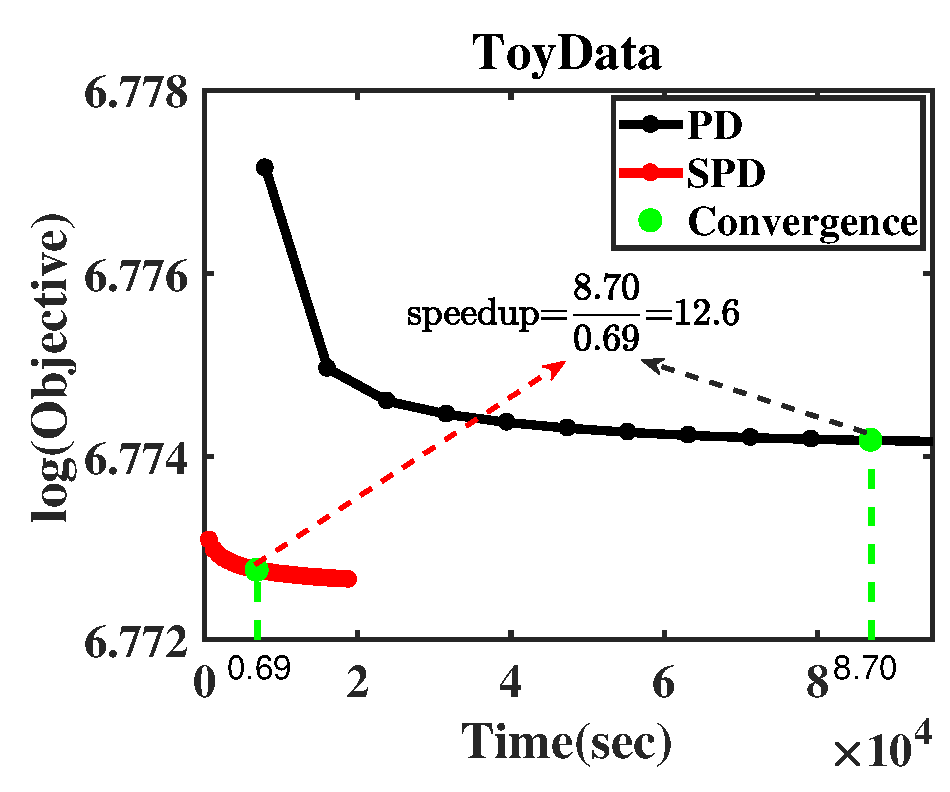
\includegraphics[width=0.7\textwidth]{ToyDataset_Objective}
    \caption{PD和SPD算法在ToyData上的收敛对比}
    \label{fig:ToyDataset_Objective}
\end{figure}
图\ref{fig:ToyDataset_Objective}表明,就收敛速度而言,SPD算法显著由于PD算法。在我们的评估中,SPD算法相比PD算法会有大概12.6倍的加速比。而且,在每一轮迭代,虽然PD算法的目标函数下降得更多,但是我们的随机方法相比批处理方法使用更少的训练时间。这是因为在每一轮迭代更新的时候,PD算法使用所有的数据去进行一个精确的更新,而SPD算法只使用一小部分样本去进行一个近似的更新。当训练一个大规模的网络数据时,由于计算效率和内存限制的原因,PD算法将会比SPD算法花费更多的时间来使用一轮数据集进行更新。因此,在处理大规模网络数据时,SPD算法的收敛速度会比PD算法快很多。这同时也验证了公式\eqref{eq:exponentiallyweightedmovingaverage}作为损失函数的优点:一个算法无需花费太多的时间去精确地最小化经验损失。另外,就像梯度下降一样,PD算法同样遭遇局部极小值问题,而SPD算法可以更好地避免该问题,从而能够收敛到一个更小的局部极小值。


\subsection{在MCG-WEBV和YKS上对比PD和SPD}

对于话题排序效果,图\ref{fig:cmp-accuracy}使用$Accuracy$ v.s. $FPPT$在MCG-WEBV和YKS数据集上对比了PD算法和SPD算法的结果。从图\ref{fig:cmp-accuracy}可以看出SPD算法的话题排序效果与PD算法相似。同时图\ref{fig:cmp-top10}进一步使用Top10-$F_1$ v.s. $NDT$证明了SPD算法的排序效果不比PD算法差。综上,说明我们的SPD算法可以达到和PD算法相似的话题排序效果。
\begin{figure}[!htbp]
    \centering
    \begin{subfigure}[b]{0.5\textwidth}
      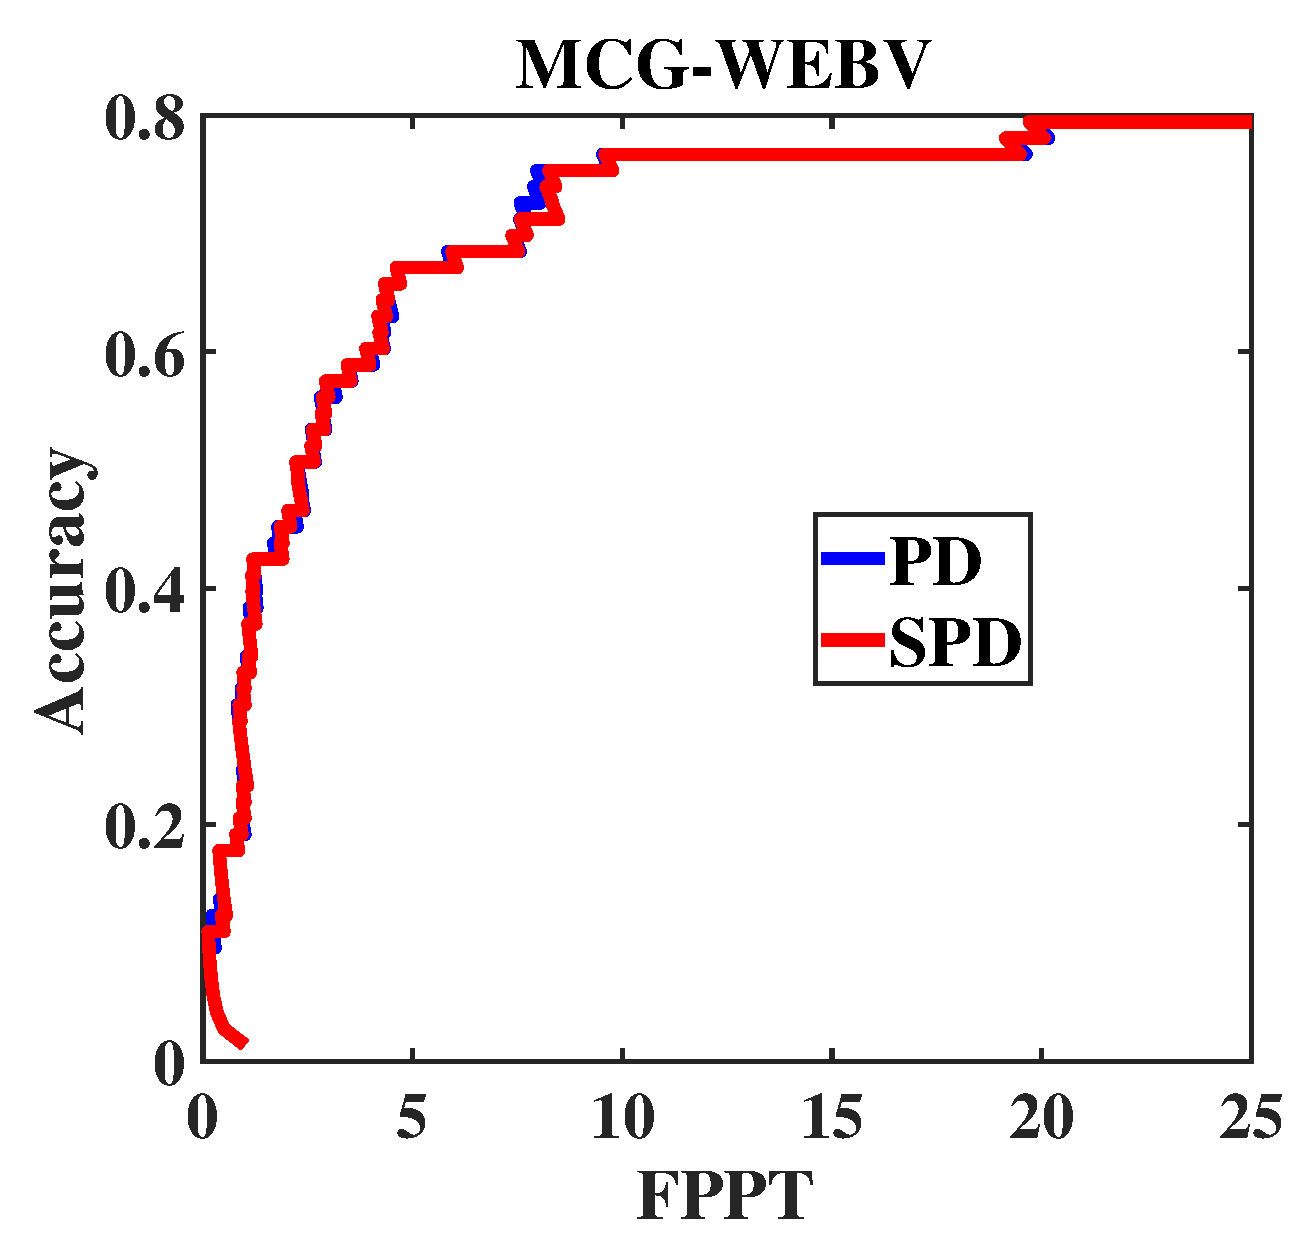
\includegraphics[width=\textwidth,height=0.95\textwidth]{MCG_Accuracy}
      \caption{}
      \label{fig:accuracycmponmcg}
    \end{subfigure}%
    \begin{subfigure}[b]{0.5\textwidth}
      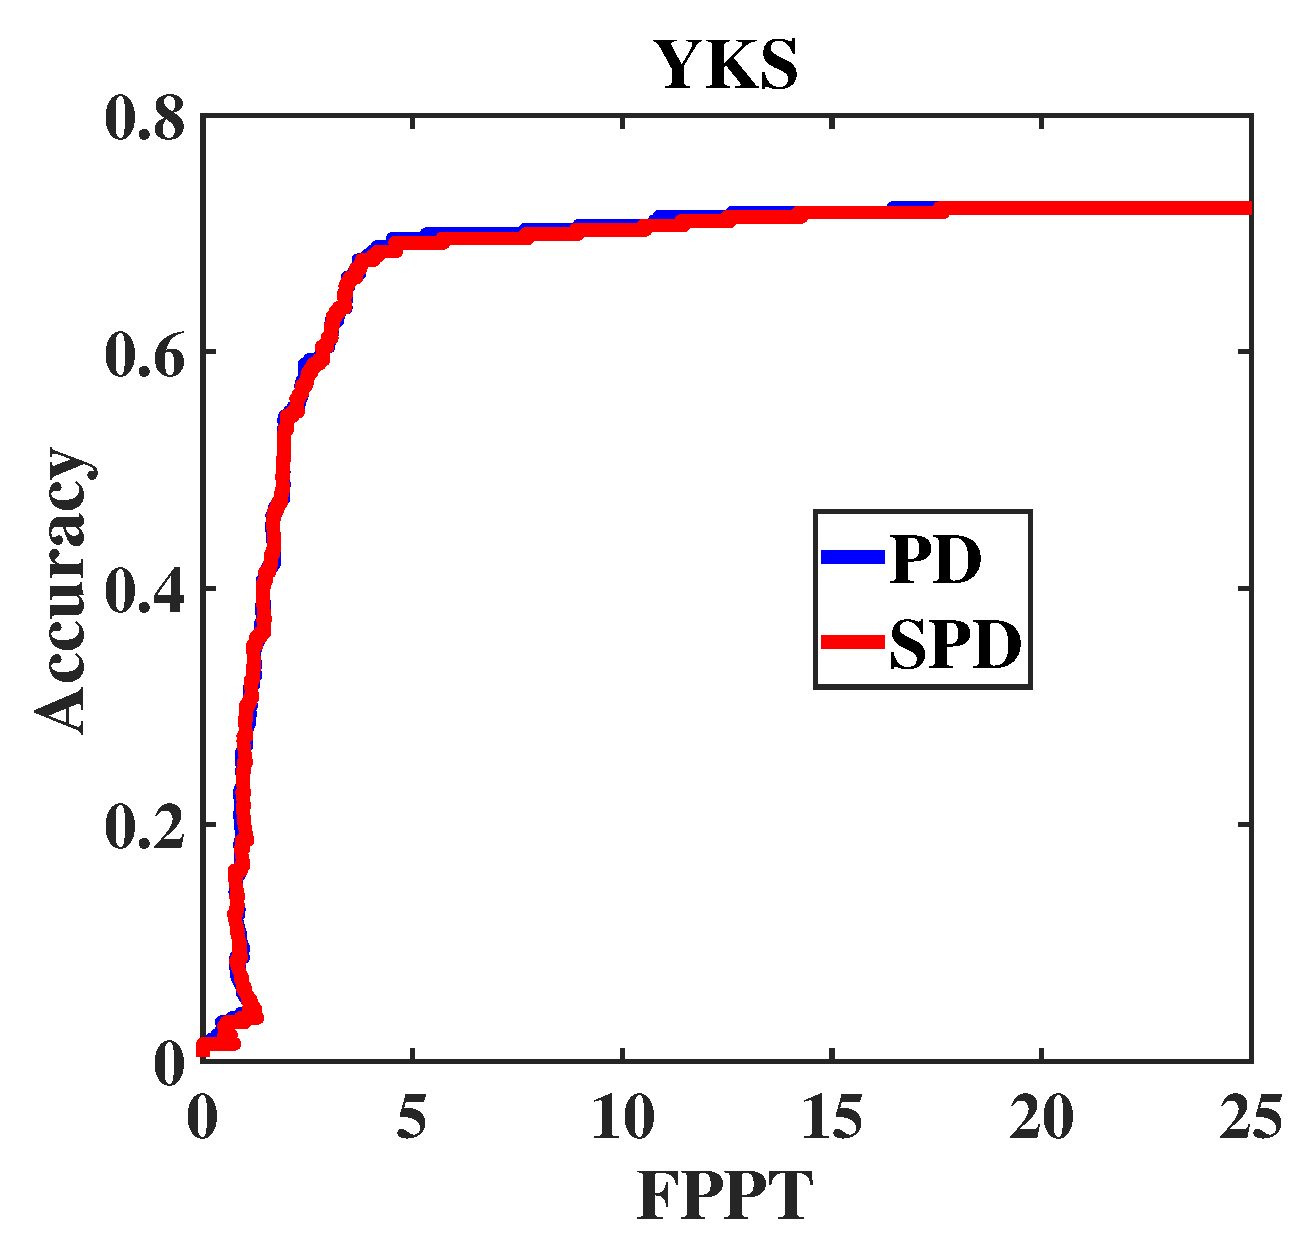
\includegraphics[width=\textwidth,height=0.95\textwidth]{YKS_Accuracy}
      \caption{}
      \label{fig:accuracycmponyks}
    \end{subfigure}%
    % ~% add desired spacing
    \caption{使用$Accuracy$ v.s. $FPPT$对比PD和SPD算法}
    \label{fig:cmp-accuracy}
\end{figure}
\begin{figure}[!htbp]
    \centering
    \begin{subfigure}[b]{0.49\textwidth}
      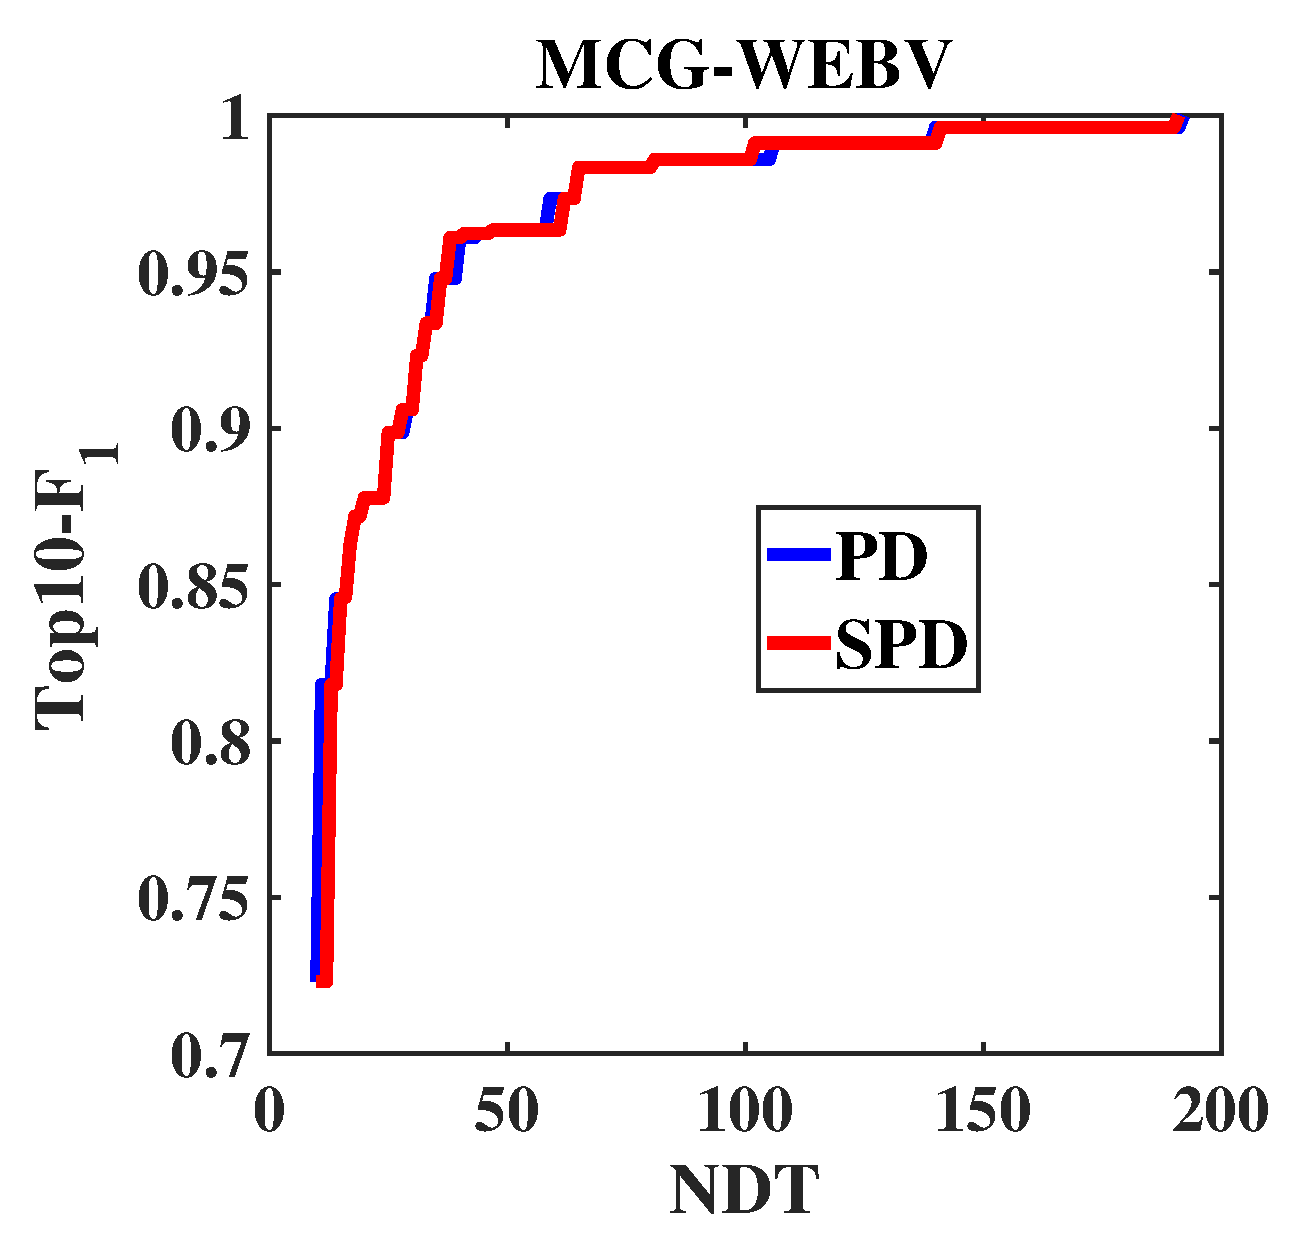
\includegraphics[width=\textwidth,height=0.95\textwidth]{MCG_Top10}
      \caption{}
      \label{fig:top10cmponmcg}
    \end{subfigure}
    % ~% add desired spacing
    \begin{subfigure}[b]{0.49\textwidth}
      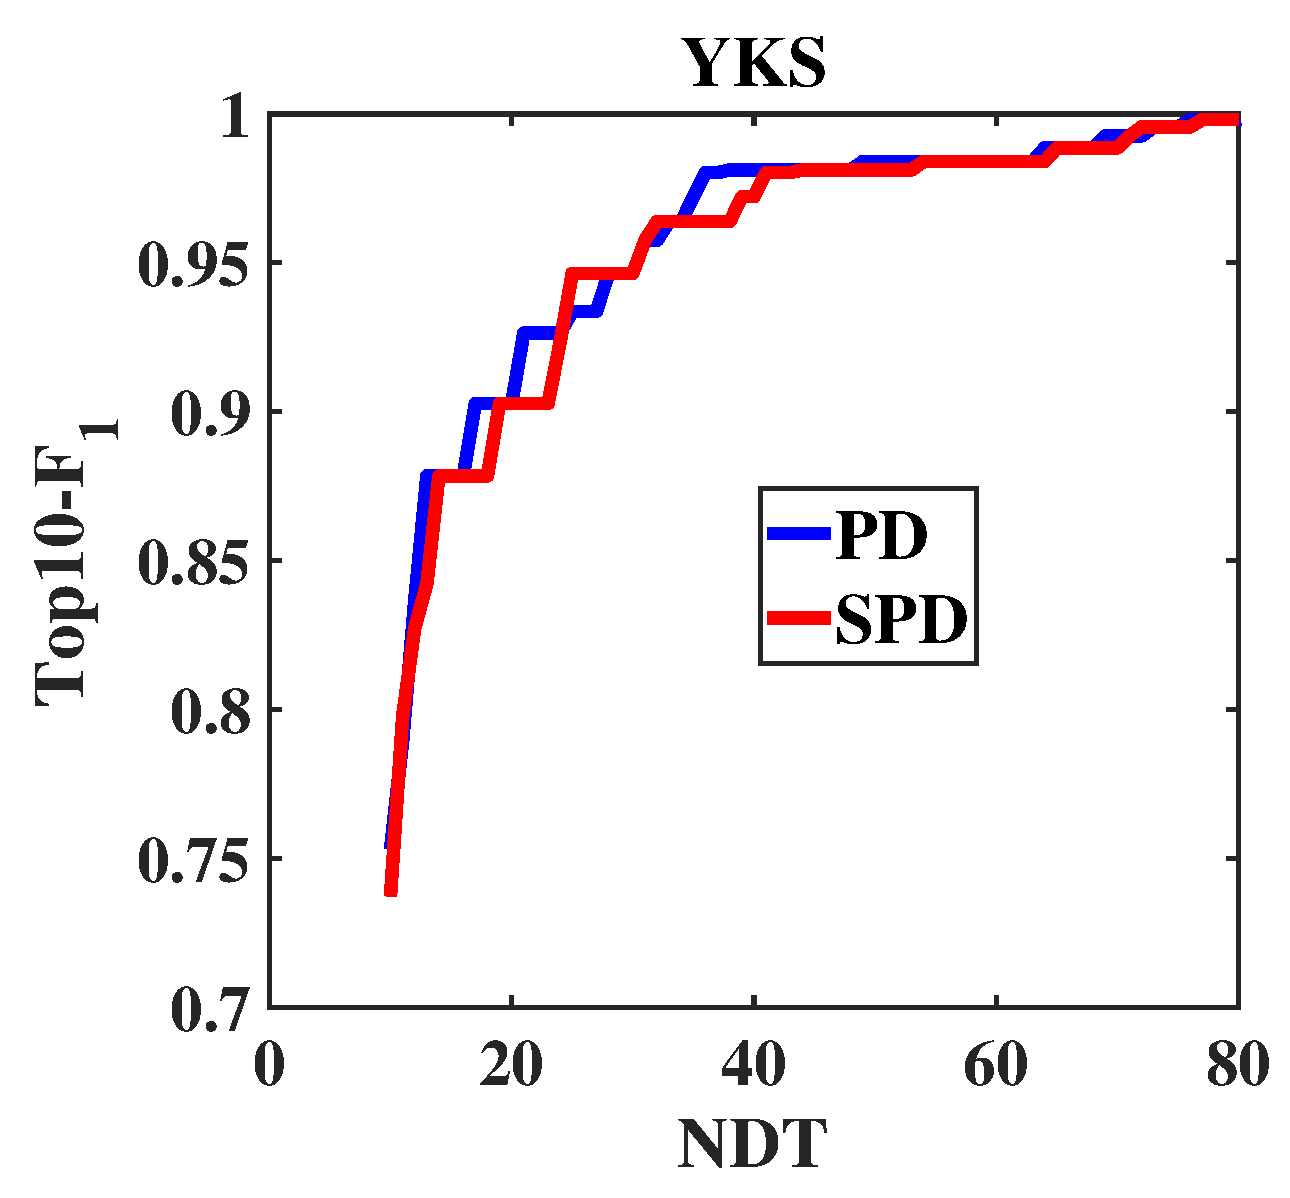
\includegraphics[width=\textwidth,height=0.95\textwidth]{YKS_Top10}
      \caption{}
      \label{fig:top10cmponyks}
    \end{subfigure}
    \caption{使用Top10-$F_1$ v.s. $NDT$对比PD和SPD算法}
    \label{fig:cmp-top10}
\end{figure}

对于话题排序效率,图\ref{fig:cmp-objective}对比PD算法和SPD算法在MCG-WEBV和YKS数据集上的收敛情况。从这两幅图中可以看出SPD算法可以收敛到一个更低的对数似然函数值。这意味这SPD算法可以在保证算法排序效果的同时使目标函数收敛到更低的值。但是由于这两个数据集都很小,SPD算法的随机采样优势没能发挥出来,所以导致SPD算法训练一遍数据集花费的时间比PD算法多。所以在处理小规模网络数据时,SPD算法收敛会比PD算法慢。但是,在处理大规模网络数据时,SPD算法的随机优势就能得以发挥使其收敛速度比PD算法快。
\begin{figure}[!htbp]
    \centering
    \begin{subfigure}[b]{0.5\textwidth}
      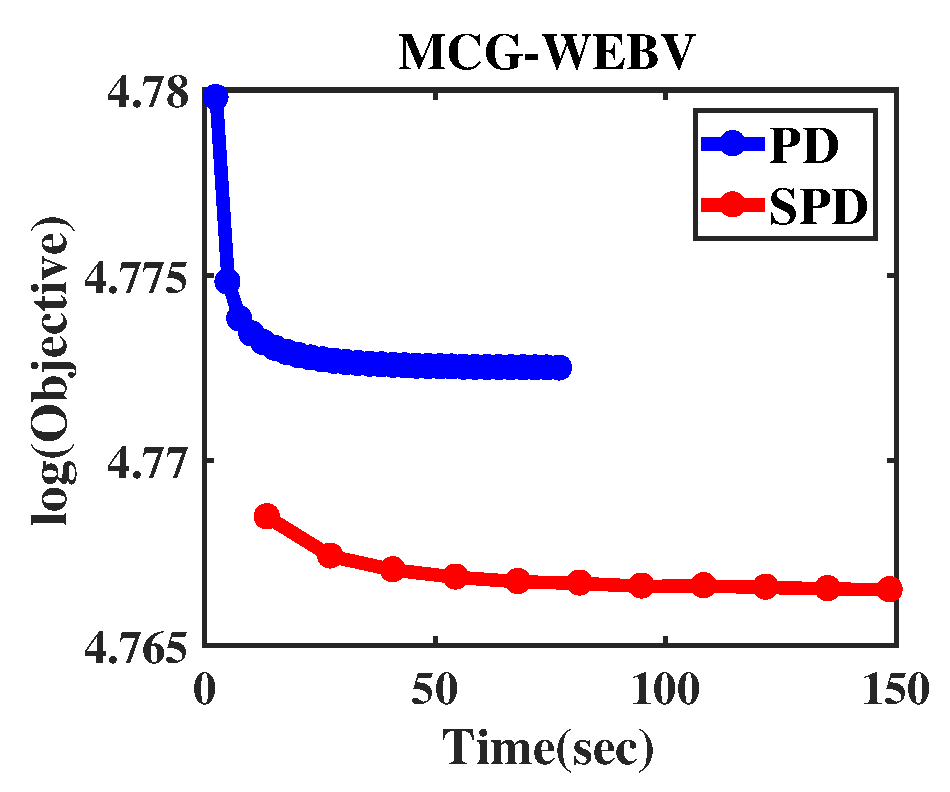
\includegraphics[width=\textwidth,height=0.95\textwidth]{MCG_Objective}
      \caption{}
      \label{fig:objectivecmponmcg}
    \end{subfigure}%
    \begin{subfigure}[b]{0.5\textwidth}
      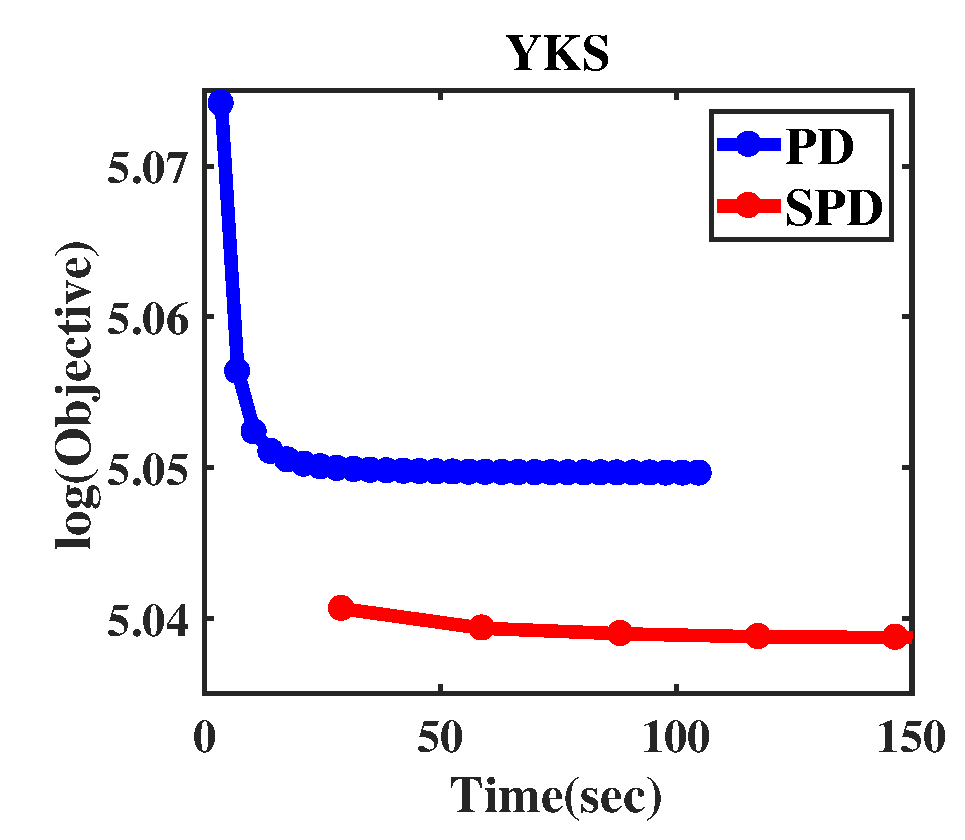
\includegraphics[width=\textwidth,height=0.95\textwidth]{YKS_Objective}
      \caption{}
      \label{fig:objectivecmponyks}
    \end{subfigure}%
    \caption{使用目标函数收敛曲线对比PD和SPD算法}
    \label{fig:cmp-objective}
\end{figure}


\subsection{参数分析}

\subsubsection{批样本数量$b$:}

图\ref{fig:minibatch-Objective}展示了在MCG-WEBV数据集上,不同的批样本数量$b$的大小对SPD算法目标函数收敛曲线的影响。从中可以看出不同的批样本数量$b$均收敛到一个局部极小值。此外,$b$值越小,对数目标函数值也会收敛到更低的程度。一个可能的解释是更小的批样本数量会带来更大的随机性,使得SPD算法更有可能逃离较差的局部极小值,到达一个相对较好的局部极小值。
\begin{figure}[!htbp]
    \centering
    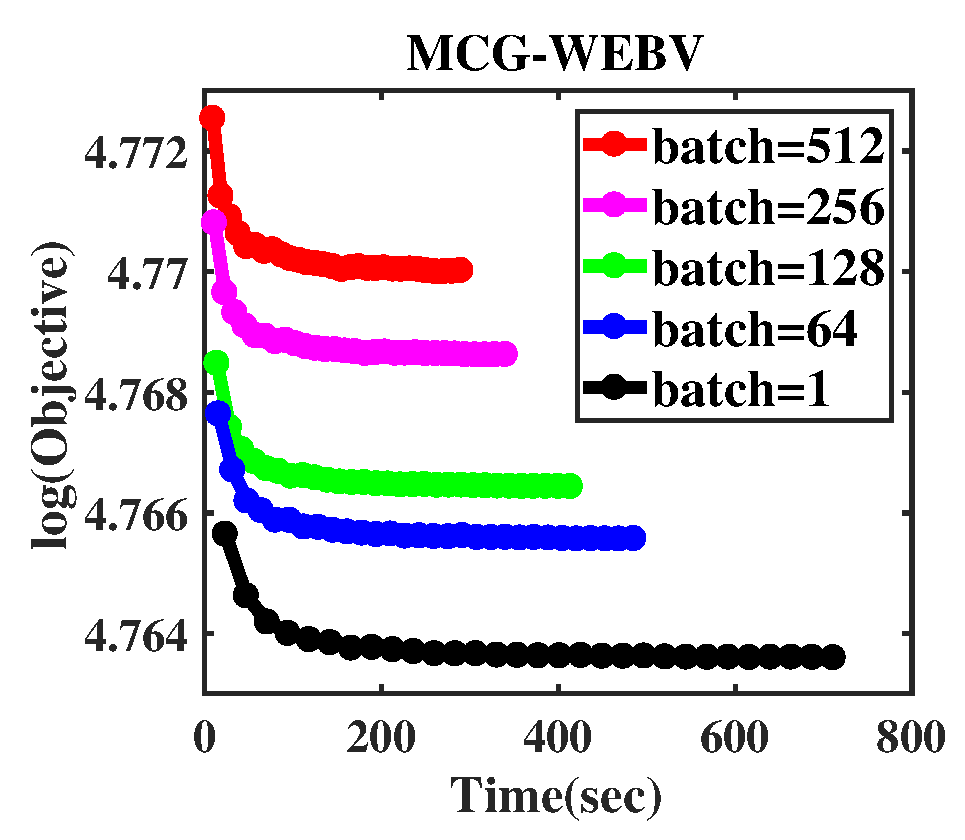
\includegraphics[width=0.7\textwidth]{minibatch_Objective}
    \caption{不同批样本数量$b$对目标函数收敛曲线的影响}
    \label{fig:minibatch-Objective}
\end{figure}

有趣的是,图\ref{fig:minibatch-two-metric}显示不同大小的批样本数量均能获得相似的$Accuracy$和Top10-$F_1$值。可能的原因是即使不同的$b$值导致最终的话题权重$\mu$值的分布不同,对数目标函数值不同。但是,只要这些话题权重$mu$值的相对大小分布几乎不变,即对$\mu$值排序后的所处位置在不同批样本数量时几乎不变,那么就有可能达到相似的$Accuracy$和Top10-$F_1$。因此,批样本数量$b$的大小不会影响SPD算法的话题排序性能。
\begin{figure}[!htbp]
    \centering
    \begin{subfigure}[b]{0.5\textwidth}
      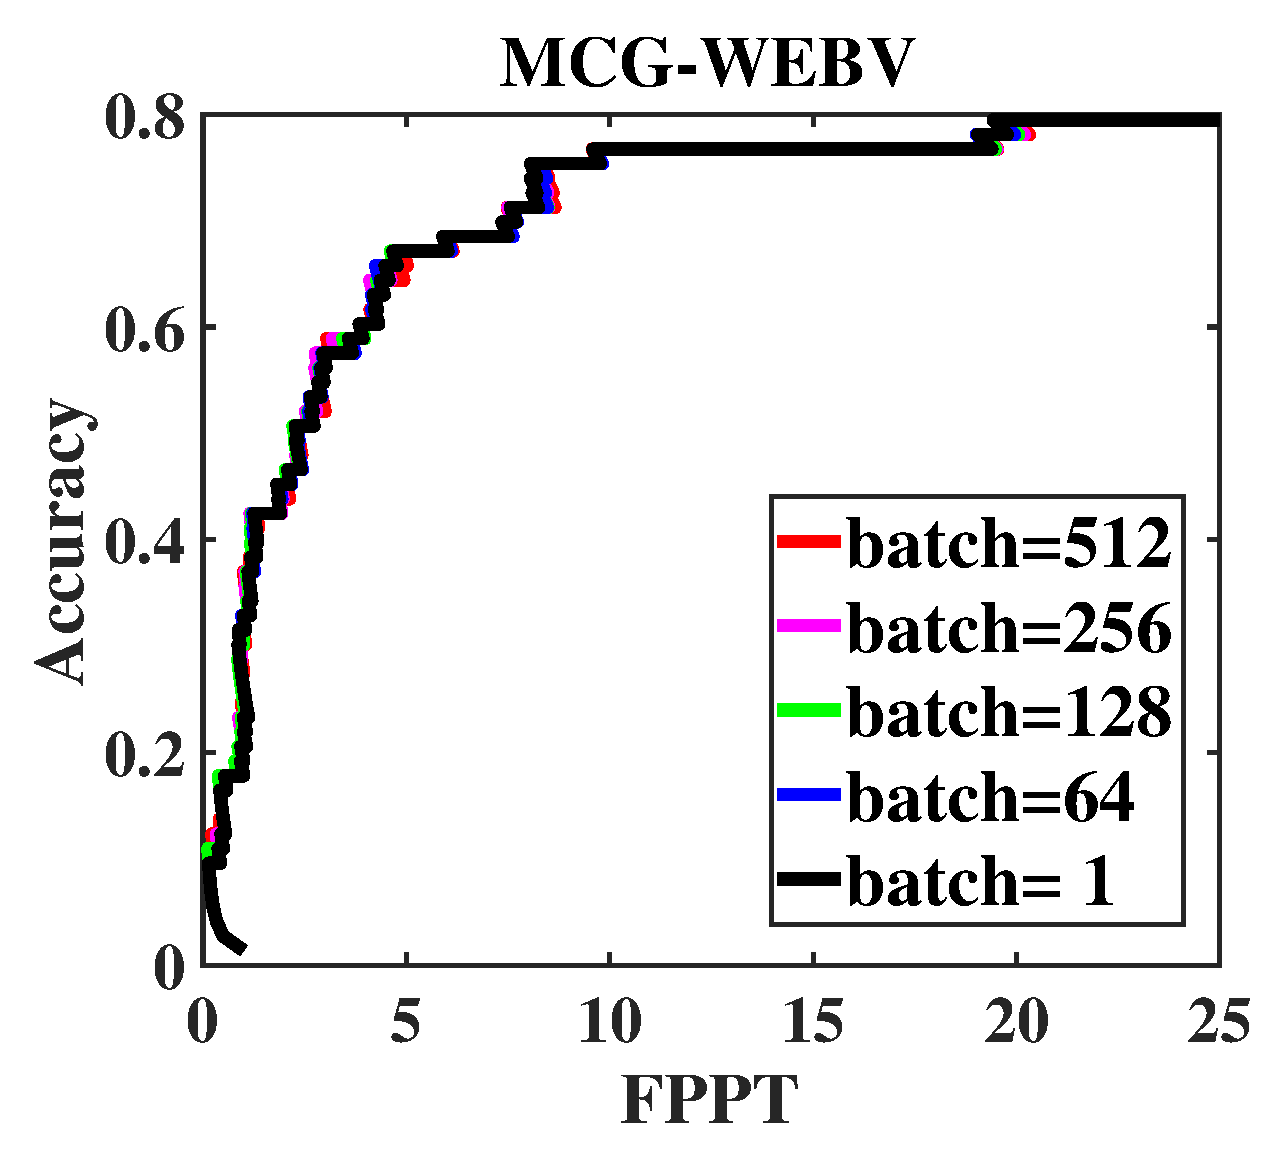
\includegraphics[width=\textwidth,height=0.95\textwidth]{minibatch_Accuracy}
      \caption{}
      \label{fig:minibatch_Accuracy}
    \end{subfigure}%
    % ~% add desired spacing
    \begin{subfigure}[b]{0.5\textwidth}
      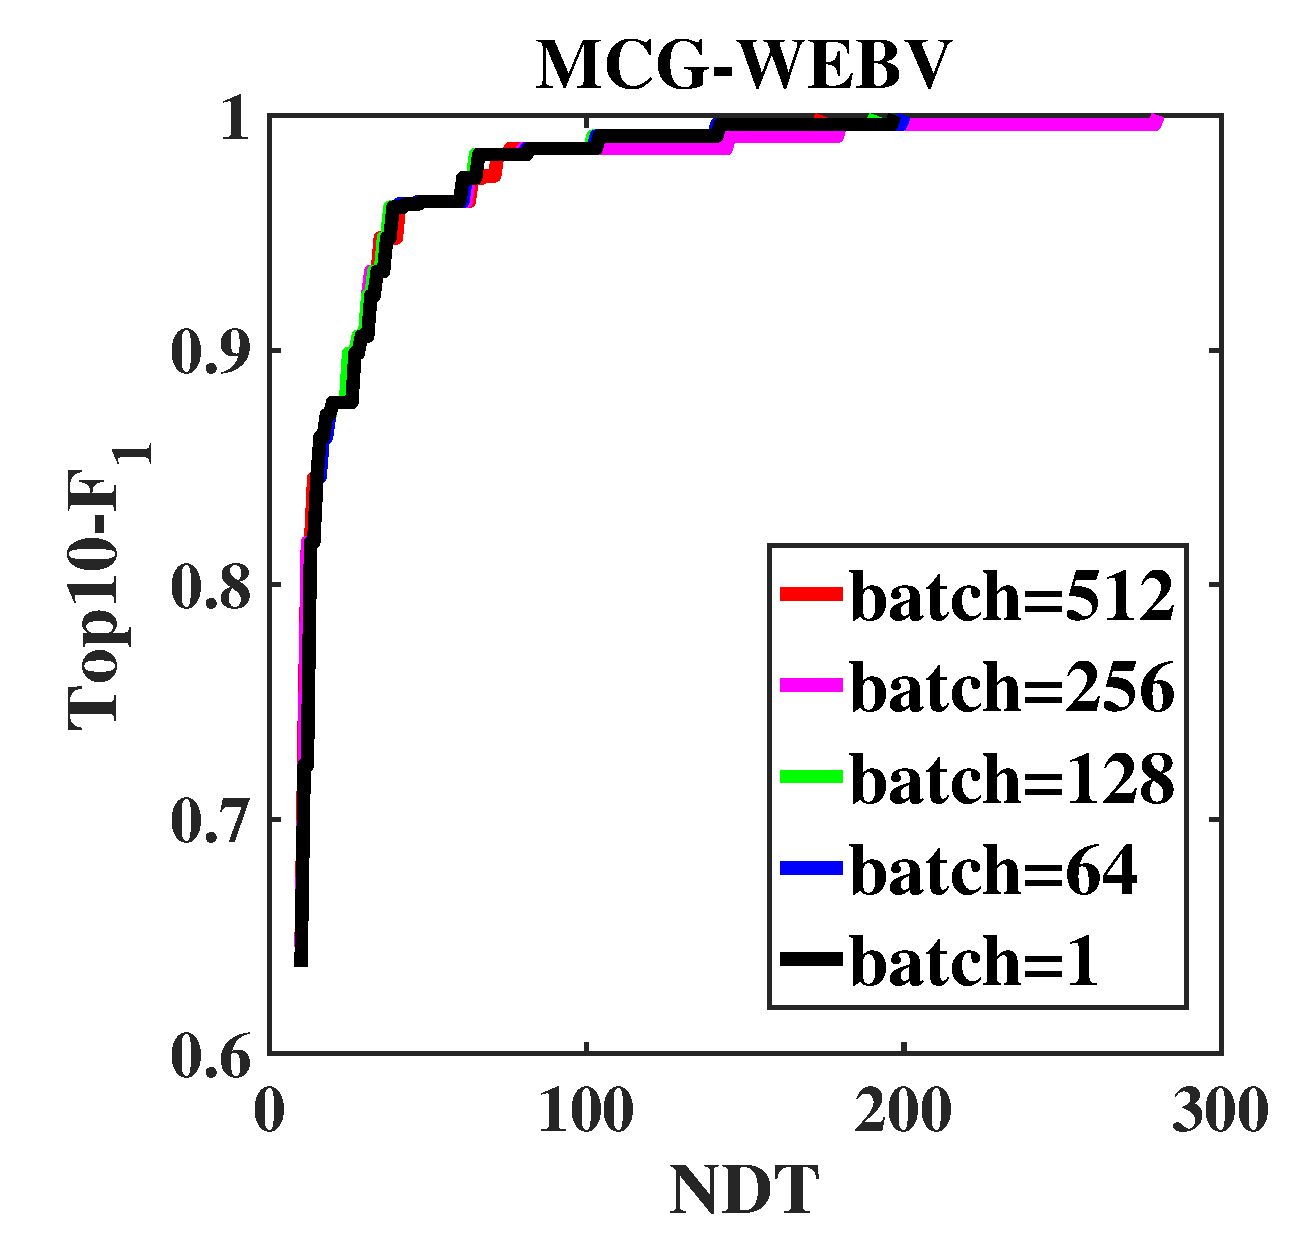
\includegraphics[width=\textwidth,height=0.95\textwidth]{minibatch_Top10}
      \caption{}
      \label{fig:minibatch_Top10}
    \end{subfigure}
    \caption{不同批样本数量$b$的话题排序效果对比}
    \label{fig:minibatch-two-metric}
\end{figure}

\subsubsection{权重参数$\alpha$和$\beta$:}

我们在公式\eqref{eq:weightupdate}使用了一个衰减权重。其中$\beta$是一个初始权重,$\alpha$是一个权重衰减因子。

图\ref{fig:Objective_Beta}展示了当固定其他参数(比如:$\alpha=0$,$b=128$,$T=30$),不同$\beta$值在收敛速度上的对比。正如所预期的那样,$\beta$越大,SPD算法的收敛速度越快。这是因为一个较大的$\beta$值使得近似代理函数能够快速适应当前最新的代理函数。
\begin{figure}[!htbp]
    \centering
    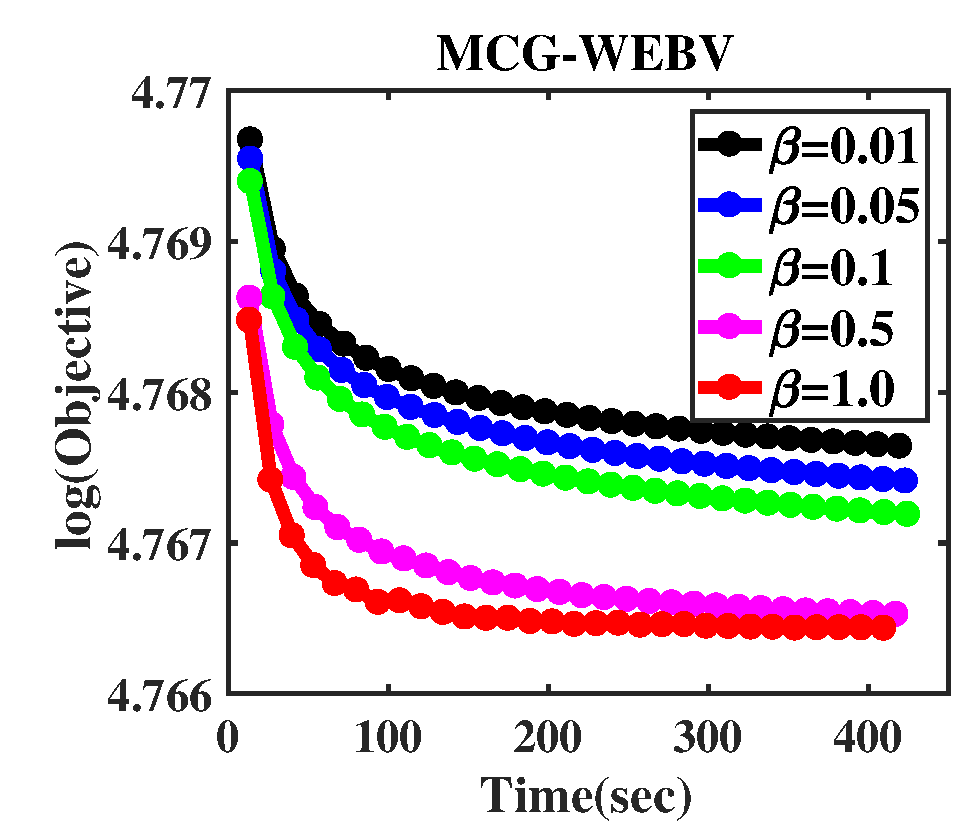
\includegraphics[width=0.7\textwidth]{Objective_Beta}
    \caption{不同$\beta$值对目标函数收敛曲线的影响}
    \label{fig:Objective_Beta}
\end{figure}

从图\ref{fig:differentbeta}的结果中,我们发现一个较大的$\beta$值不仅会带来更快的收敛速度,而且也会带来更好的话题排序效果。
\begin{figure}[!htbp]
    \centering
    \begin{subfigure}[b]{0.5\textwidth}
      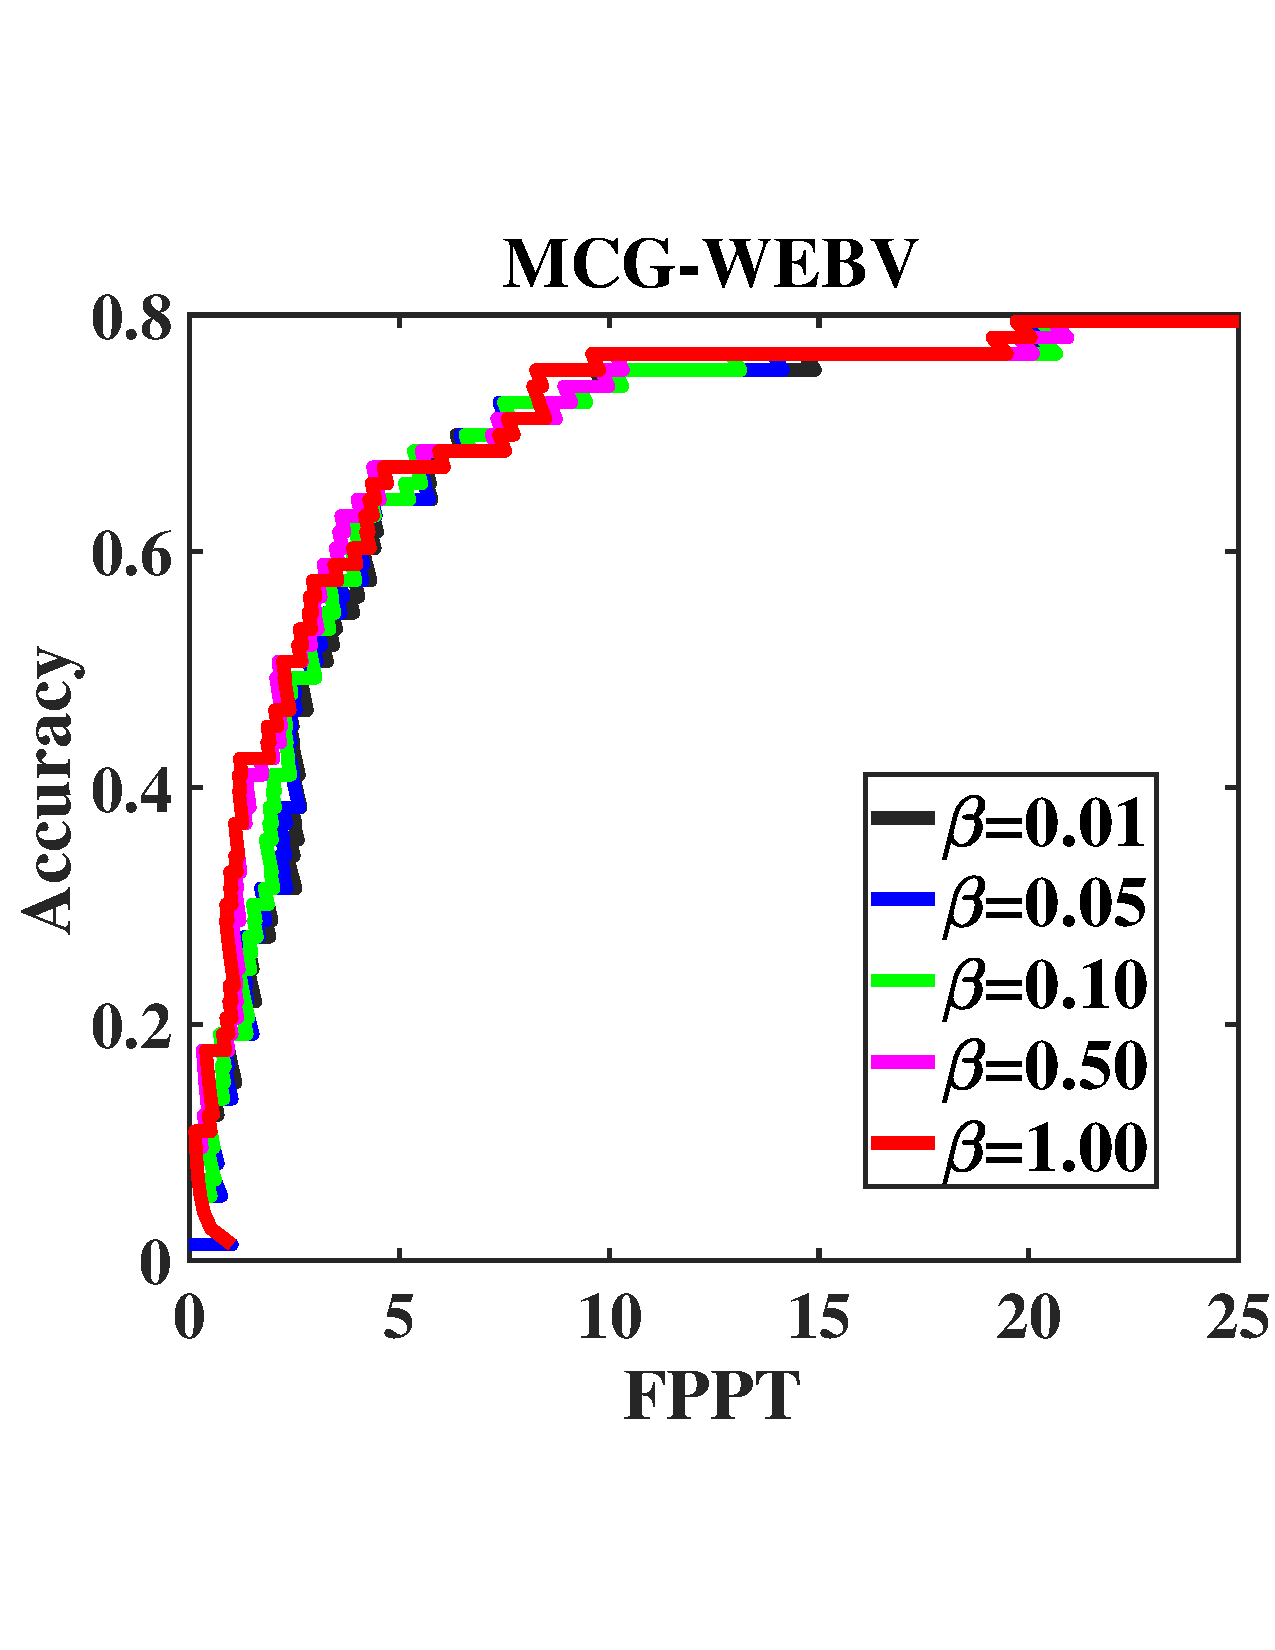
\includegraphics[width=\textwidth,height=0.95\textwidth]{Accuracy_Beta}
      \caption{}
      \label{fig:Accuracy_Beta}
    \end{subfigure}%
    % ~% add desired spacing
    \begin{subfigure}[b]{0.5\textwidth}
      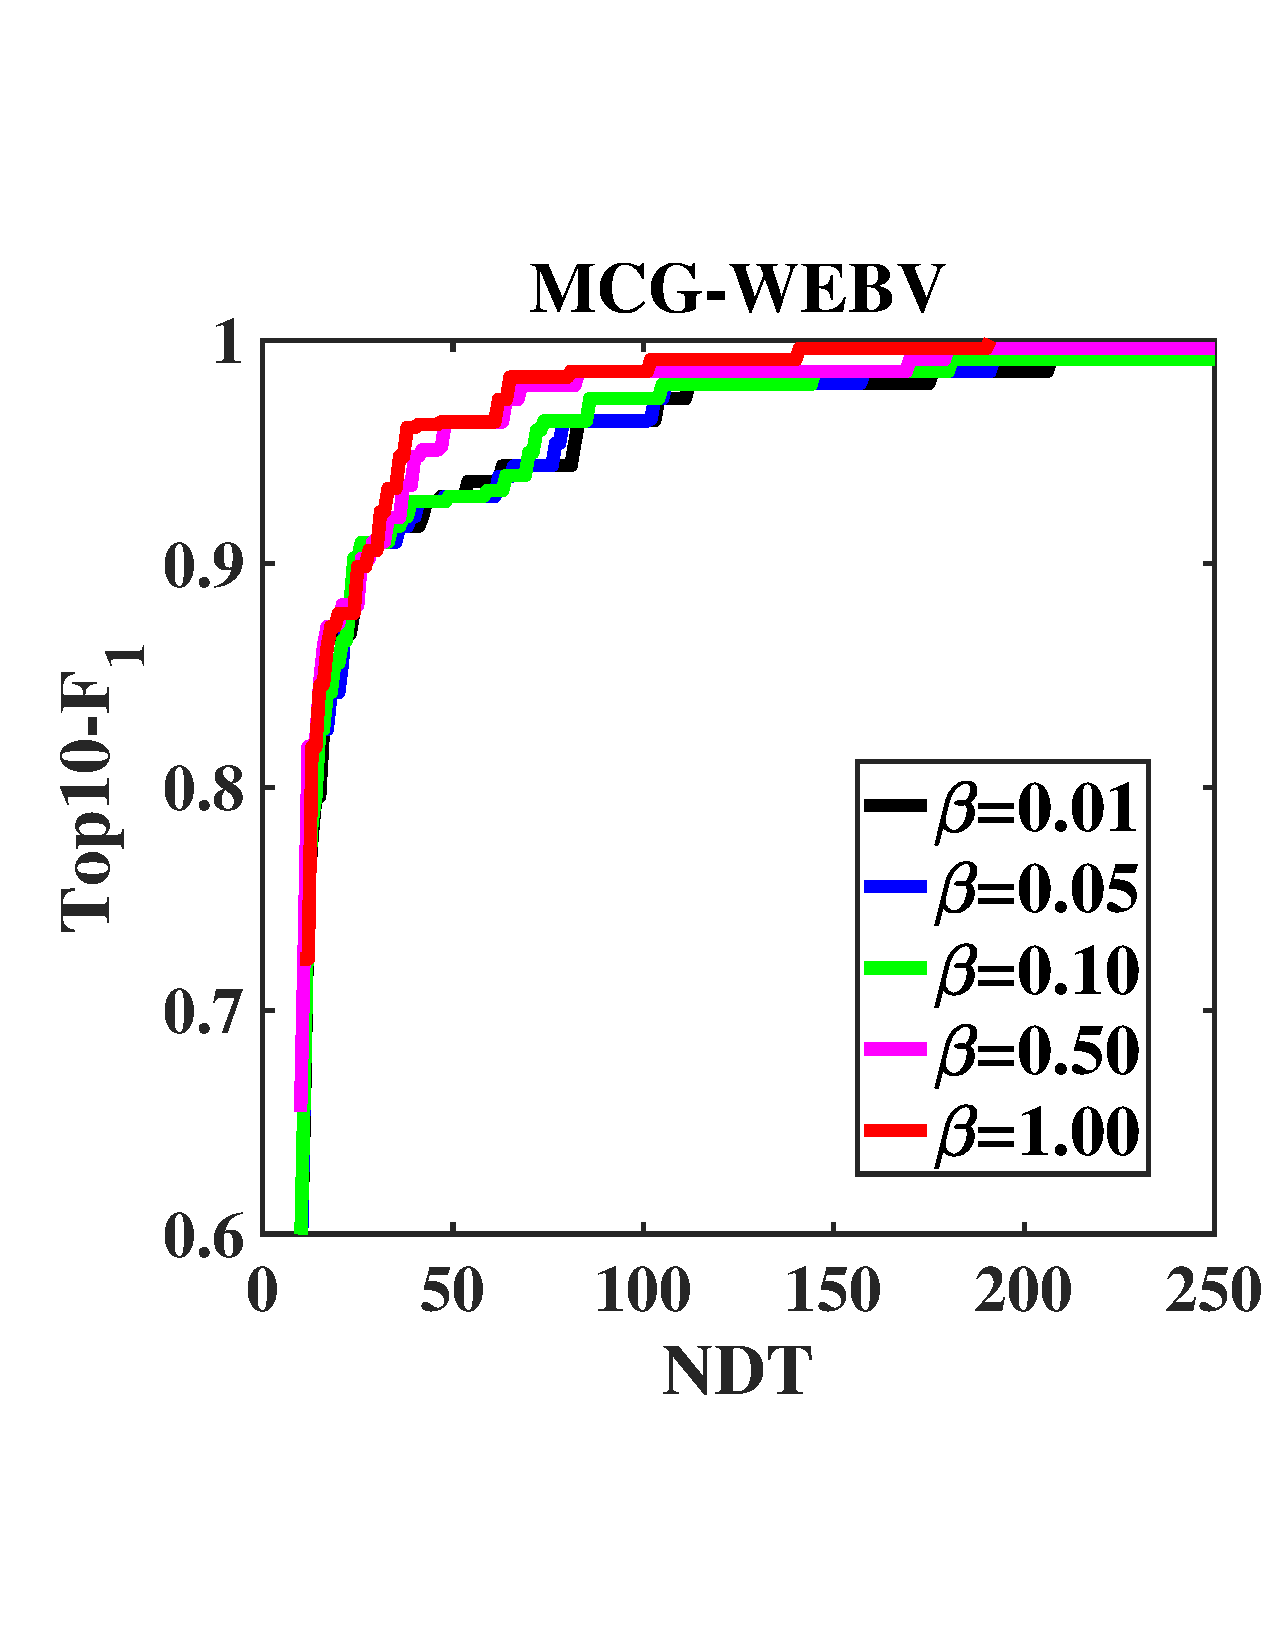
\includegraphics[width=\textwidth,height=0.95\textwidth]{Top10_Beta}
      \caption{}
      \label{fig:Top10_Beta}
    \end{subfigure}
    \caption{不同$\beta$值的话题排序效果对比}
    \label{fig:differentbeta}
\end{figure}

图\ref{fig:Objective_Alpha}展示了当固定其他参数(比如:$\beta=1$,$b=128$,$T=30$),不同$\alpha$值在收敛速度上的对比。从图中可以看出一个更小的$\alpha$会带来一个更平滑的目标函数收敛曲线。这是因为更小的$\alpha$值不仅使得$\beta$值衰减更快,而且也会使得SPD算法对于当前样本带来的代理函数更加的稳定。虽然不同$\alpha$值的收敛过程不太一样,但是最终都会收敛到一个相似的局部极小值。
\begin{figure}[!htbp]
    \centering
    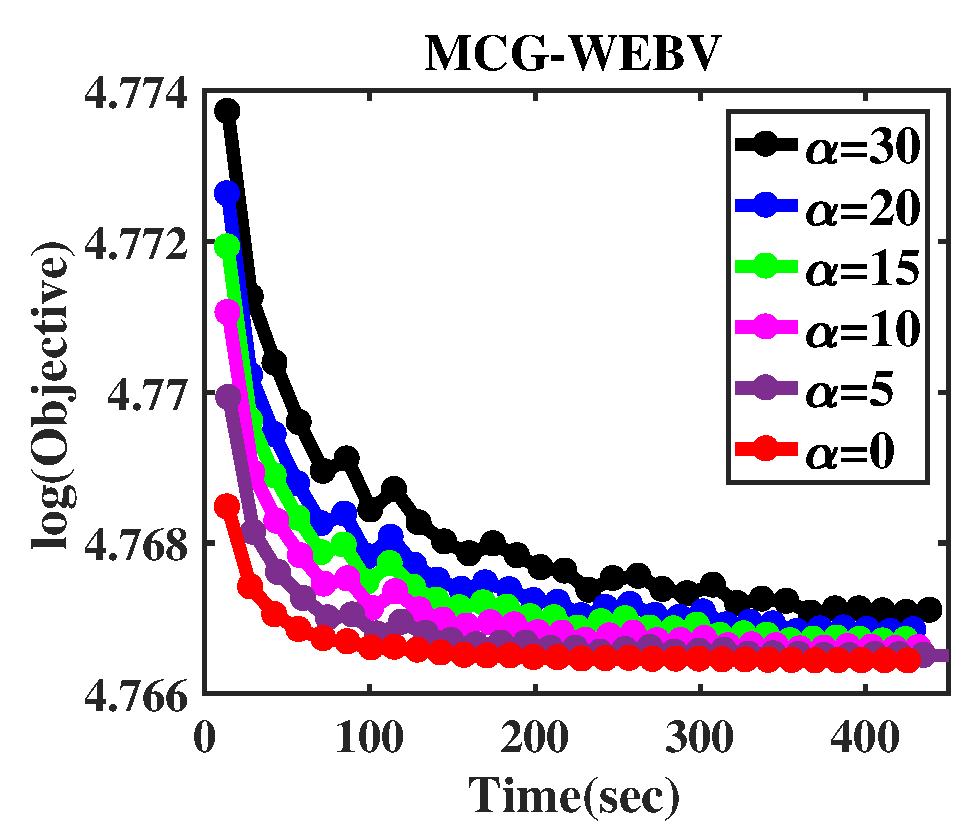
\includegraphics[width=0.7\textwidth]{Objective_Alpha}
    \caption{不同$\alpha$值对目标函数收敛曲线的影响}
    \label{fig:Objective_Alpha}
\end{figure}

从图\ref{fig:differentalpha}的结果中,可以看出不同$\alpha$值的话题排序性能几乎是一致的。
\begin{figure}[!htbp]
    \centering
    \begin{subfigure}[b]{0.5\textwidth}
      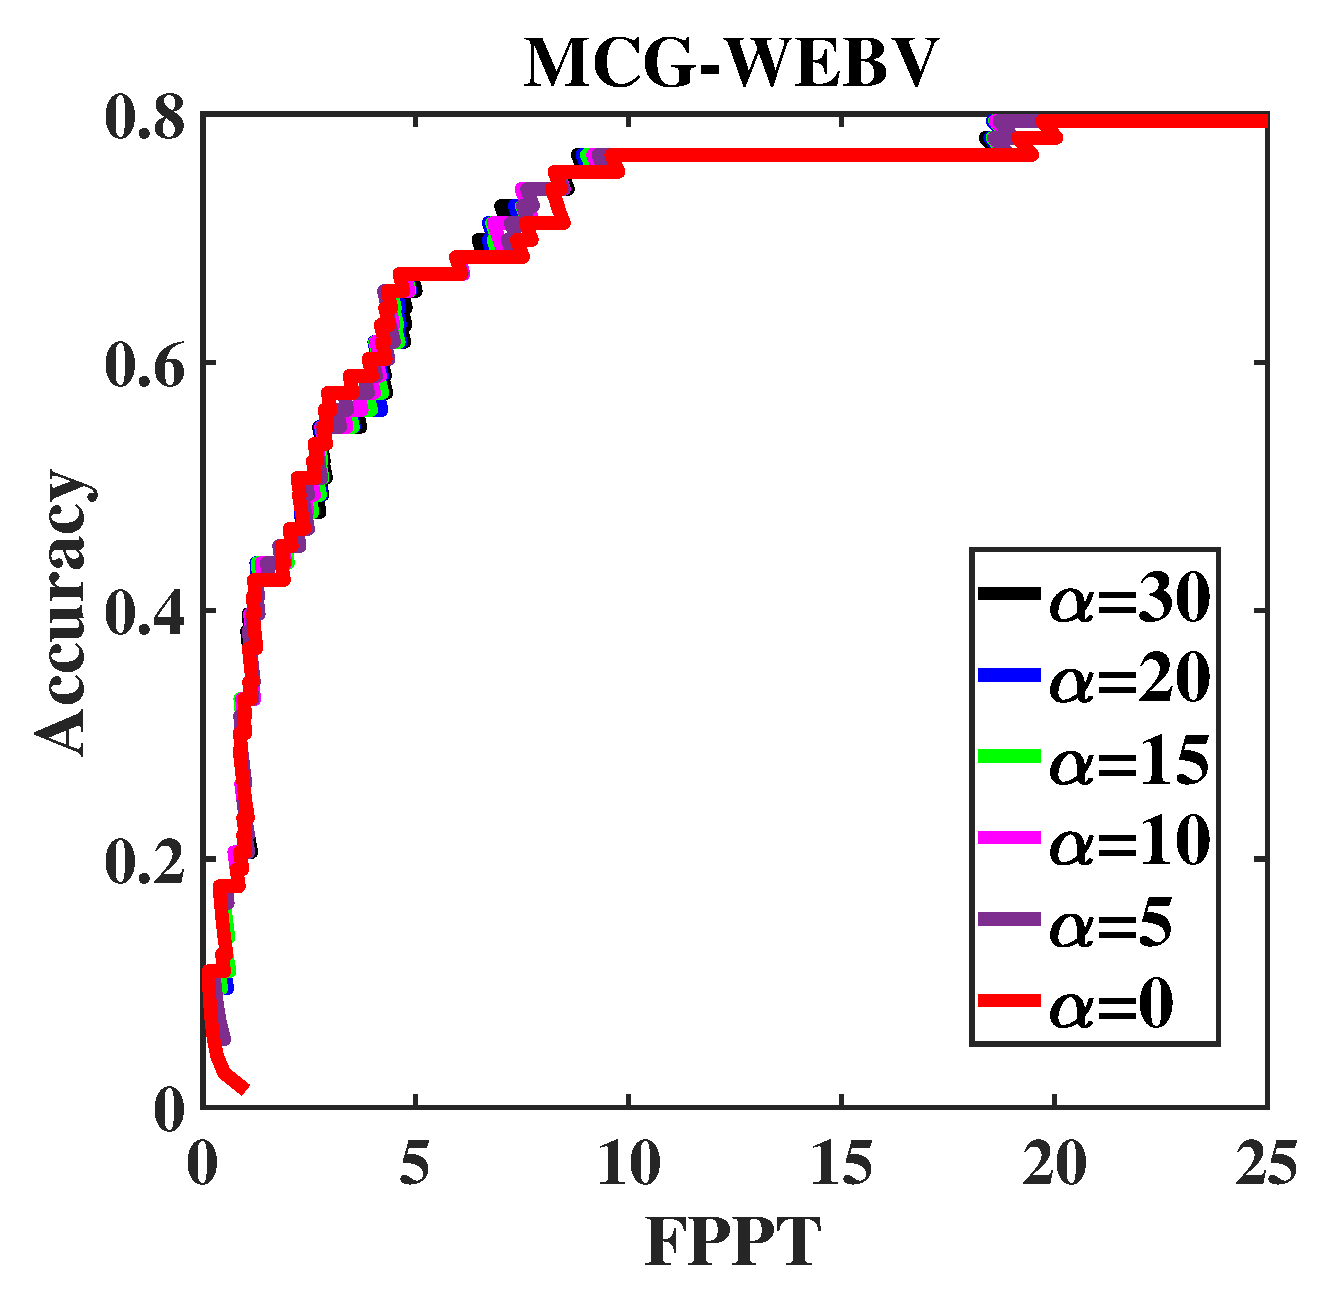
\includegraphics[width=\textwidth,height=0.95\textwidth]{Accuracy_Alpha}
      \caption{}
      \label{fig:Accuracy_Alpha}
    \end{subfigure}%
    % ~% add desired spacing
    \begin{subfigure}[b]{0.5\textwidth}
      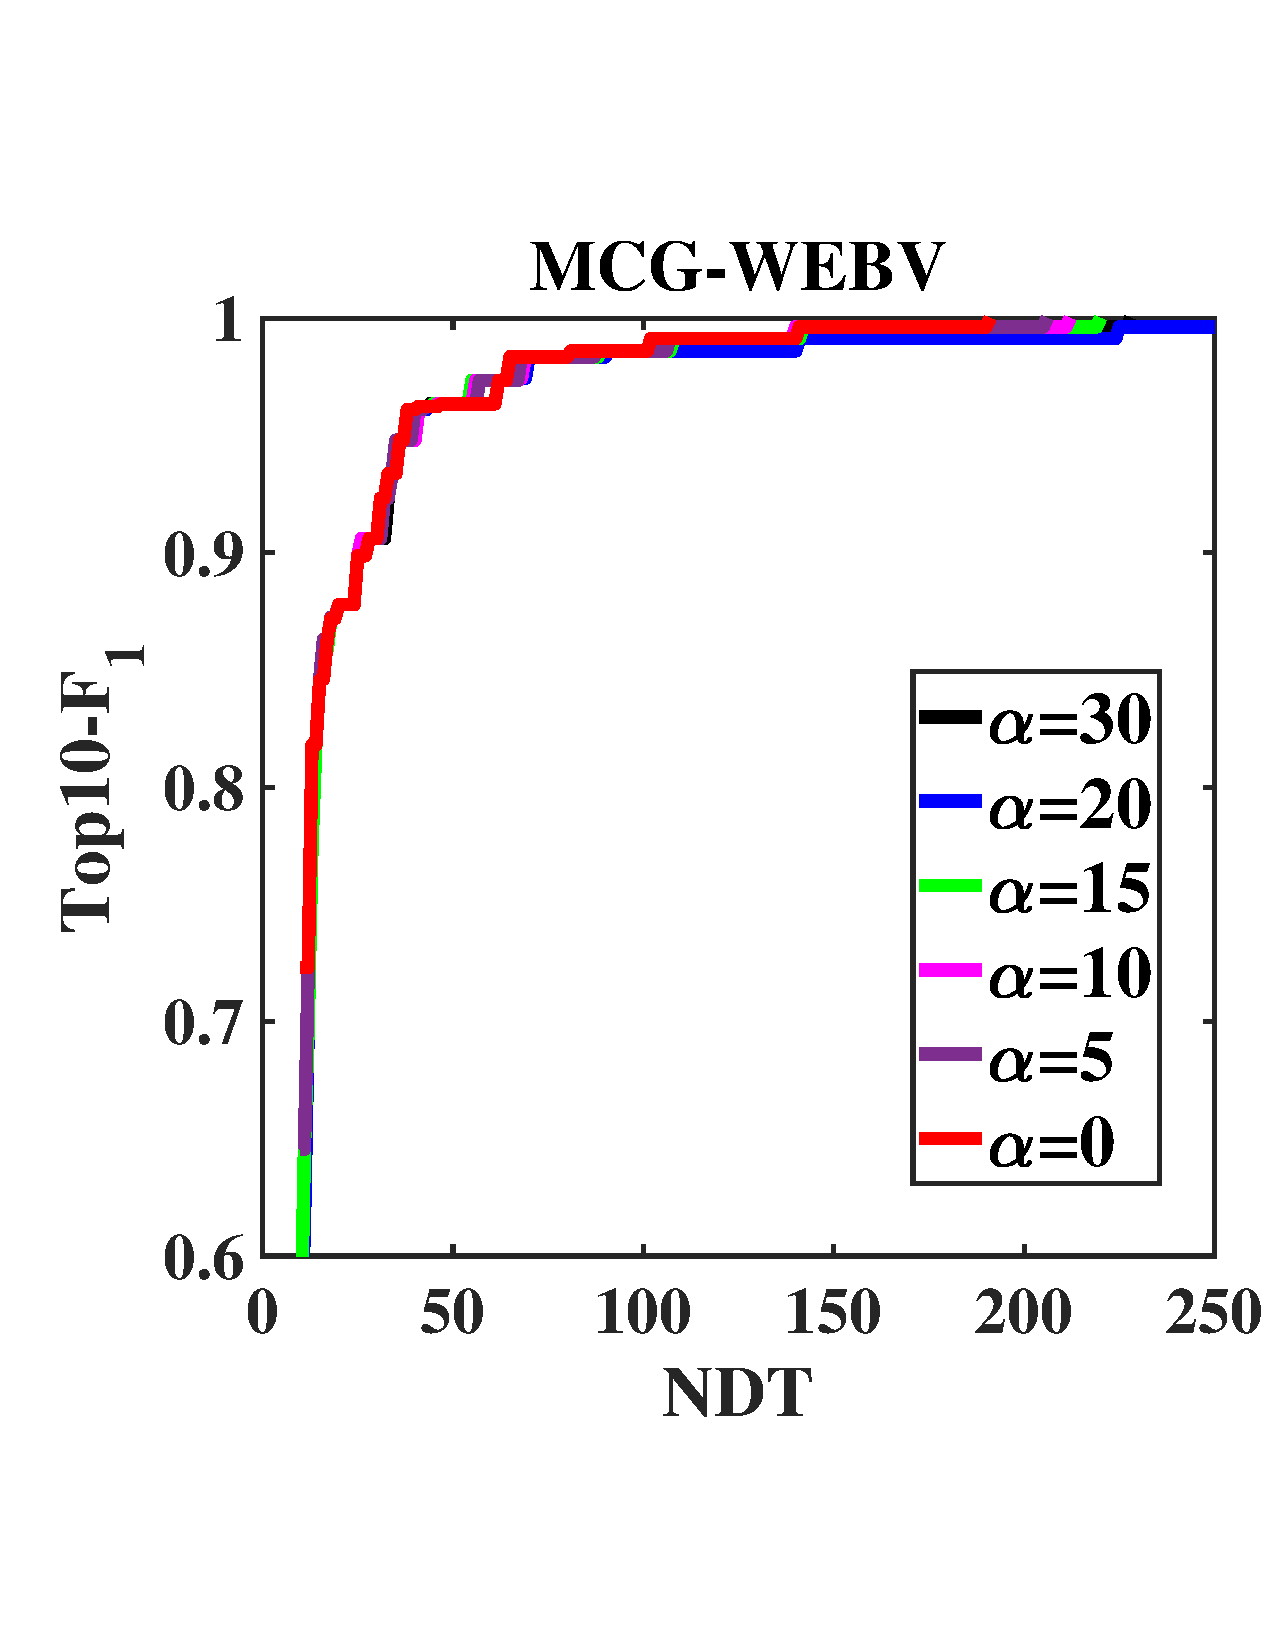
\includegraphics[width=\textwidth,height=0.95\textwidth]{Top10_Alpha}
      \caption{}
      \label{fig:Top10_Alpha}
    \end{subfigure}
    \caption{不同$\alpha$值的话题排序效果对比}
    \label{fig:differentalpha}
\end{figure}

通过以上实验结果可以得到,不同的$\alpha$和$\beta$值虽然会在一定程度上影响SPD算法中目标函数的收敛速度,但是从$Accuracy$和Top10-$F_1$来看,这些不同参数的不同取值对话题排序效果的影响不是很大。所以,可以认为我们的SPD算法是一个对参数具有鲁棒性的算法。


\subsection{异步并行实验}

我们使用python语言开了4个进程来实现AsySPD算法。图\ref{fig:ToyData_Objective_AsySPD}展示了SPD算法和AsySPD算法在人工数据集上的收敛情况。从图中可以看出,AsySPD算法相对SPD算法的加速比达到了3.3倍,证明AsySPD算法是有效的。但是AsySPD算法的收敛值比SPD算法大,这可能是因为使用了异步无锁并行策略,导致在使用相同数量样本进行更新时,样本利用率不高,且存在更新冲突,从而收敛到一个较大的局部极小值。
\begin{figure}[!htbp]
    \centering
    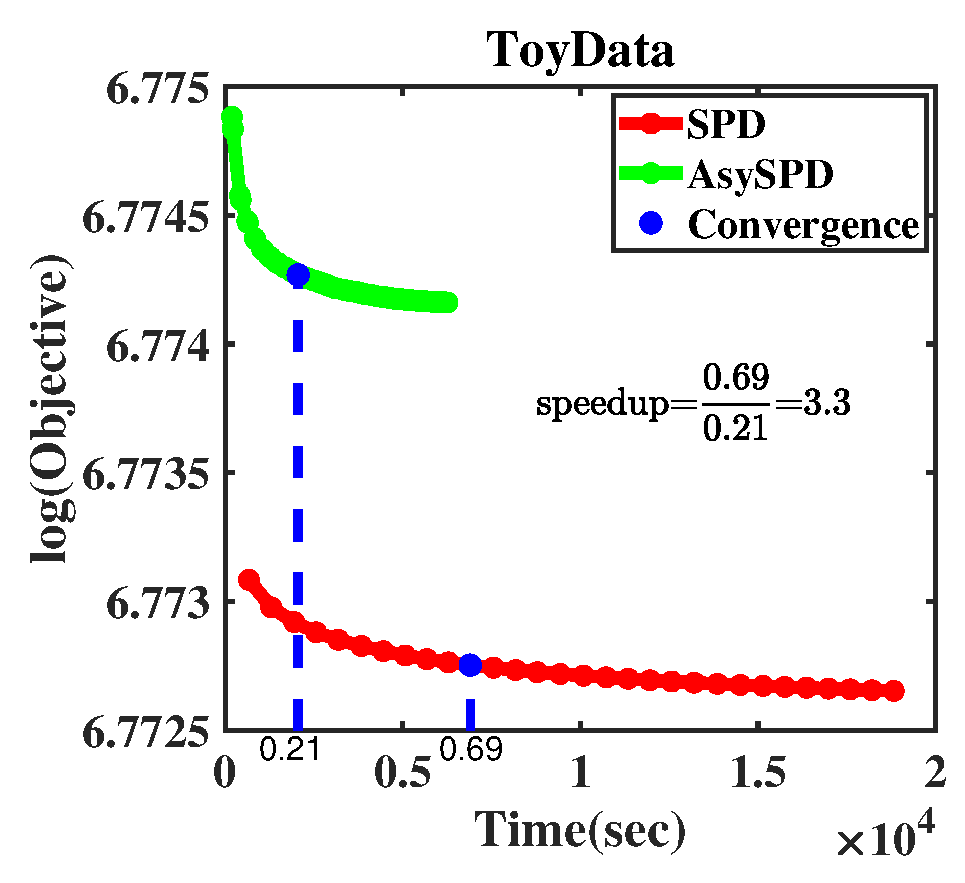
\includegraphics[width=0.7\textwidth]{ToyData_Objective_Asy}
    \caption{SPD和AsySPD算法在ToyData上的收敛对比}
    \label{fig:ToyData_Objective_AsySPD}
\end{figure}

图\ref{fig:MCG_YKS_Objective_AsySPD}展示了SPD算法和AsySPD算法在MCG-WEBV和YKS数据集上的收敛情况。同样发现AsySPD相比SPD收敛到一个较大的局部极小值。AsySPD算法的收敛趋势比较接近PD算法。
\begin{figure}[!htbp]
    \centering
    \begin{subfigure}[b]{0.5\textwidth}
      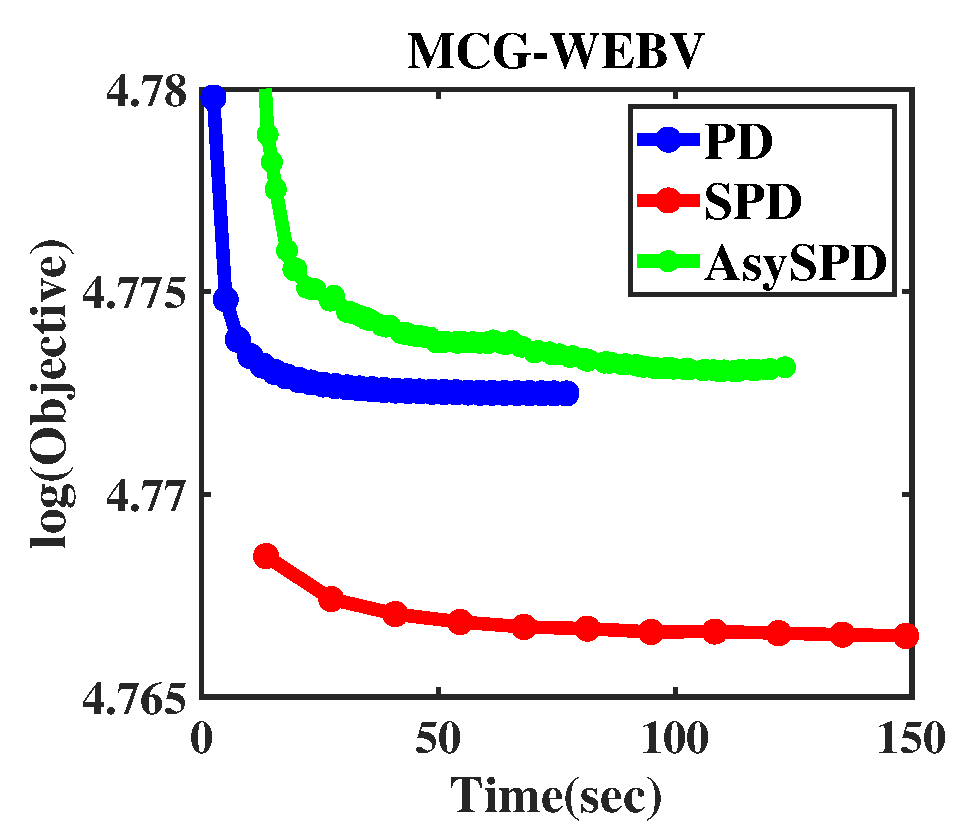
\includegraphics[width=\textwidth,height=0.95\textwidth]{MCG_Objective_Asy}
      \caption{}
      \label{fig:MCG_Objective_Asy}
    \end{subfigure}%
    % ~% add desired spacing
    \begin{subfigure}[b]{0.5\textwidth}
      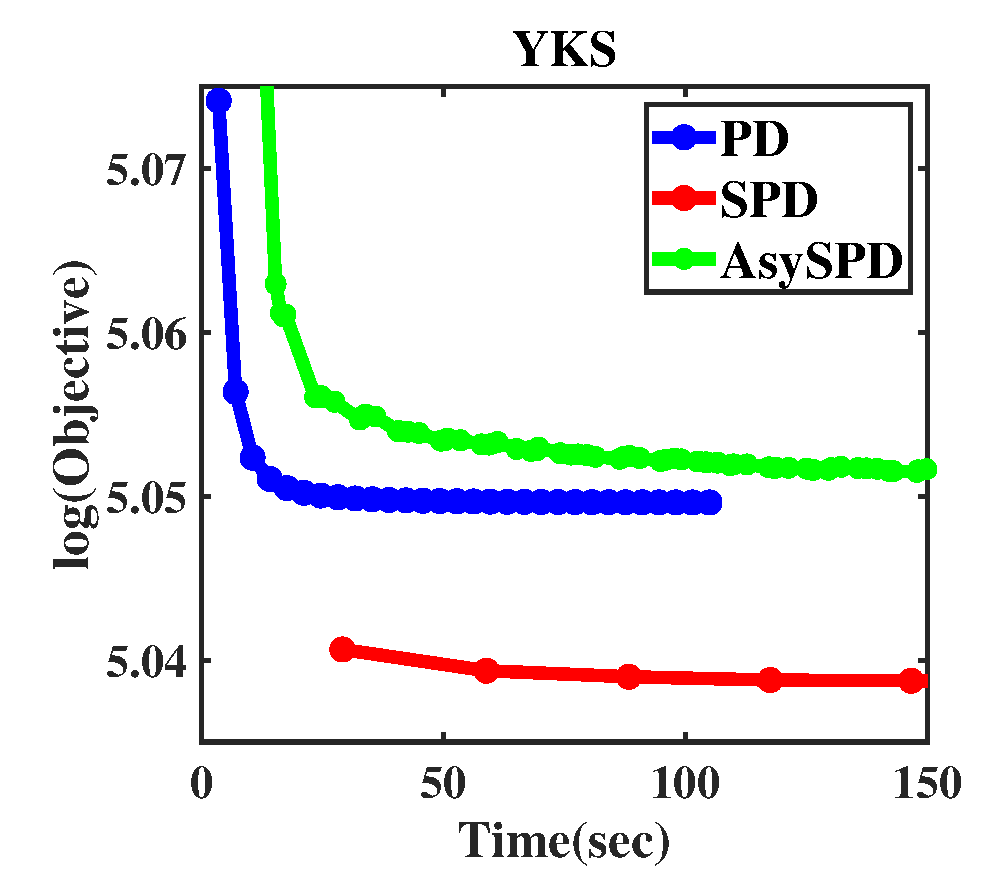
\includegraphics[width=\textwidth,height=0.95\textwidth]{YKS_Objective_Asy}
      \caption{}
      \label{fig:YKS_Objective_Asy}
    \end{subfigure}
    \caption{SPD和AsySPD算法在MCG-WEBV和YKS数据集上的收敛对比}
    \label{fig:MCG_YKS_Objective_AsySPD}
\end{figure}

\begin{figure}[!htbp]
    \centering
    \begin{subfigure}[b]{0.5\textwidth}
      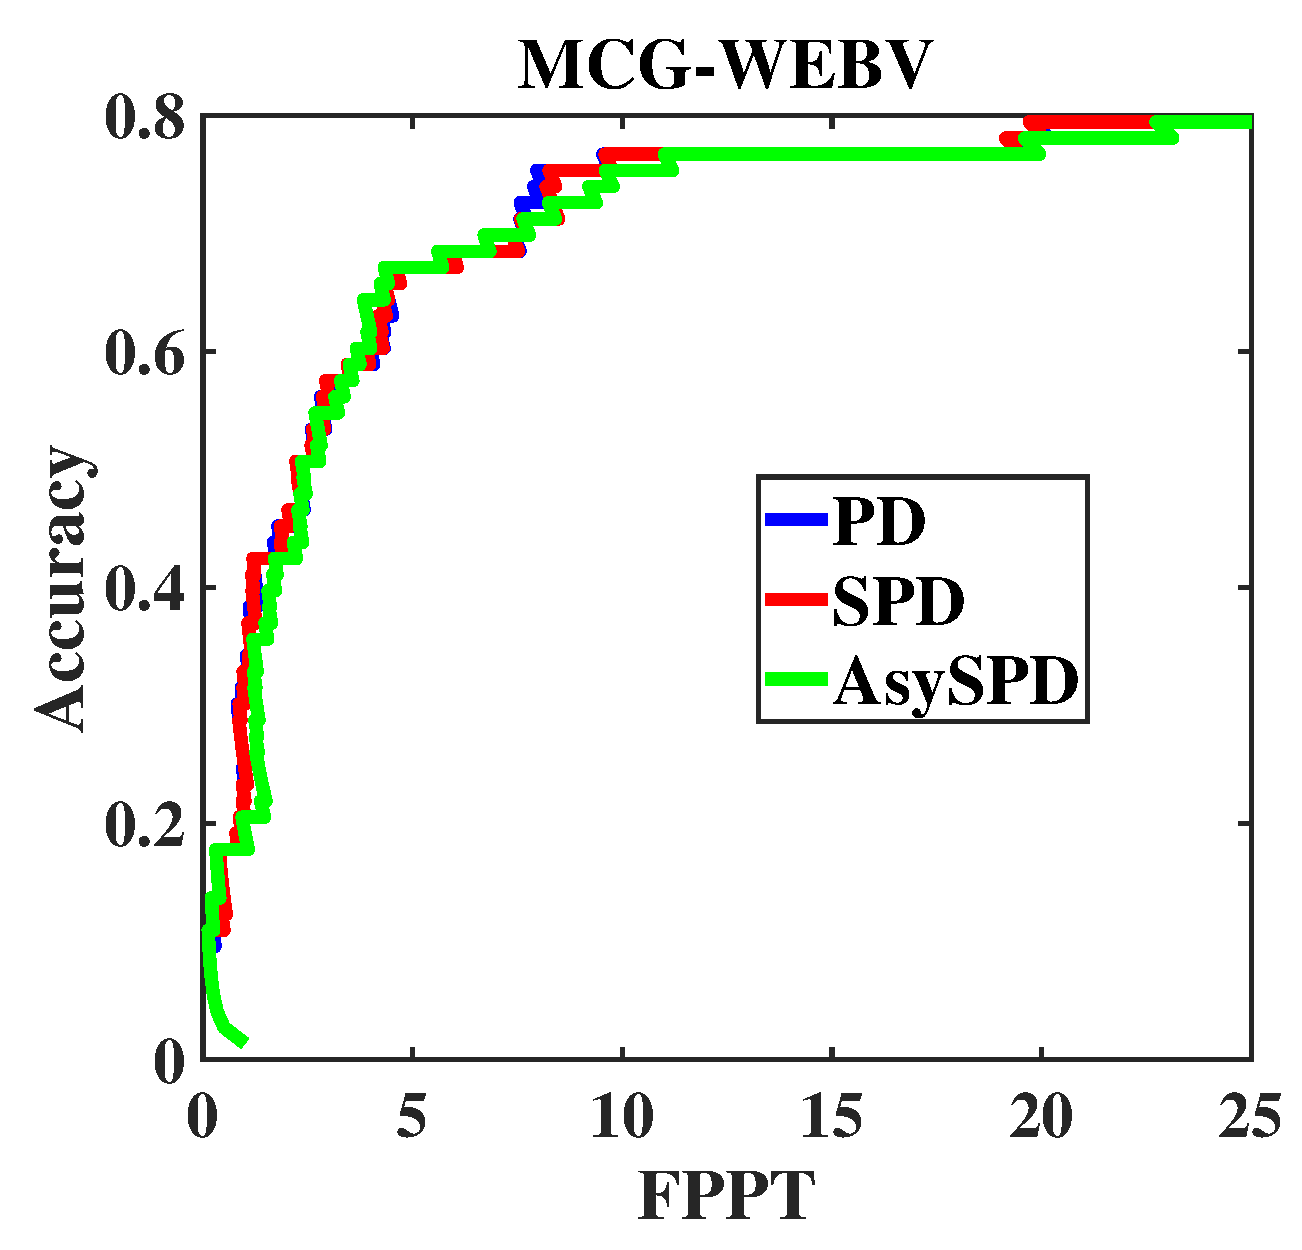
\includegraphics[width=\textwidth,height=0.95\textwidth]{MCG_Accuracy_Asy}
      \caption{}
      \label{fig:MCG_Accuracy_Asy}
    \end{subfigure}%
    % ~% add desired spacing
    \begin{subfigure}[b]{0.5\textwidth}
      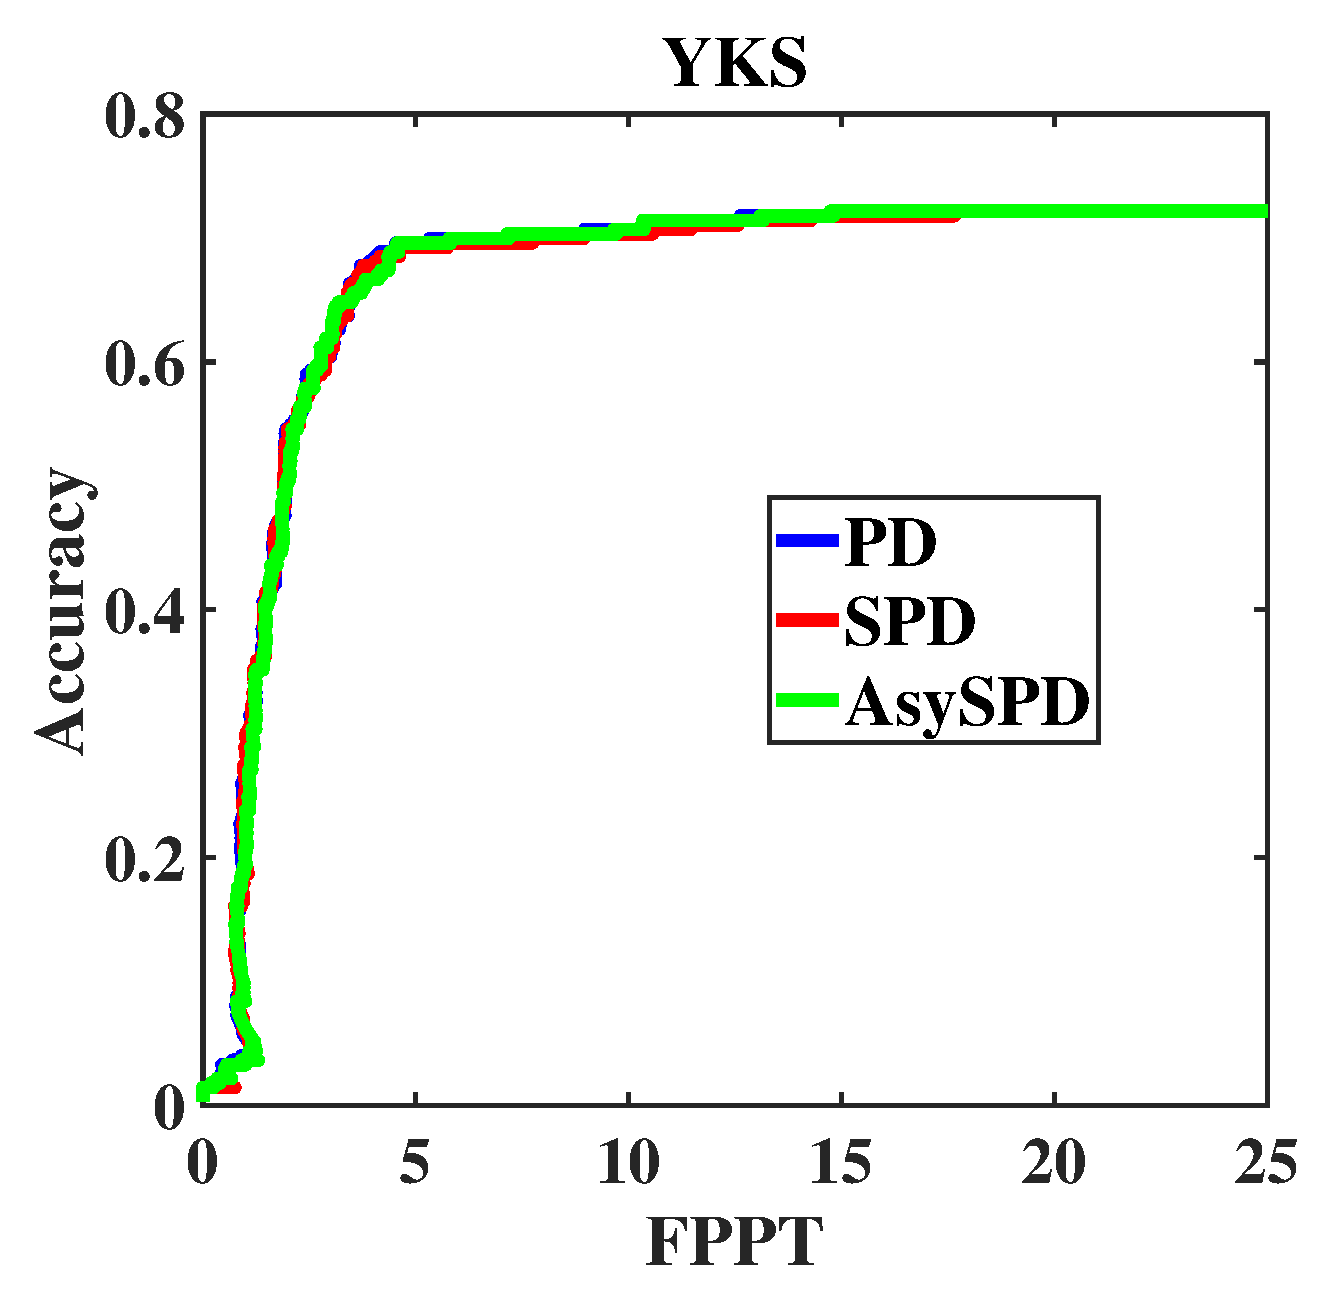
\includegraphics[width=\textwidth,height=0.95\textwidth]{YKS_Accuracy_Asy}
      \caption{}
      \label{fig:YKS_Accuracy_Asy}
    \end{subfigure}
    \caption{使用$Accuracy$ v.s. $FPPT$对比SPD和AsySPD算法}
    \label{fig:MCG_YKS_Accuracy_AsySPD}
\end{figure}
最后,我们在MCG-WEBV和YKS数据集上对比这两个算法的话题排序效果。从图\ref{fig:MCG_YKS_Accuracy_AsySPD}可以看出AsySPD算法与SPD算法在$Accuracy$上的排序上效果一致。从图\ref{fig:MCG_YKS_Top10_AsySPD}可以看出这两个算法在Top10-$F_1$的排序上效果也几乎一致。综上,实际数据集的实验结果可以经验地证明我们AsySPD算法的有效性和高效性。
\begin{figure}[!htbp]
    \centering
    \begin{subfigure}[b]{0.5\textwidth}
      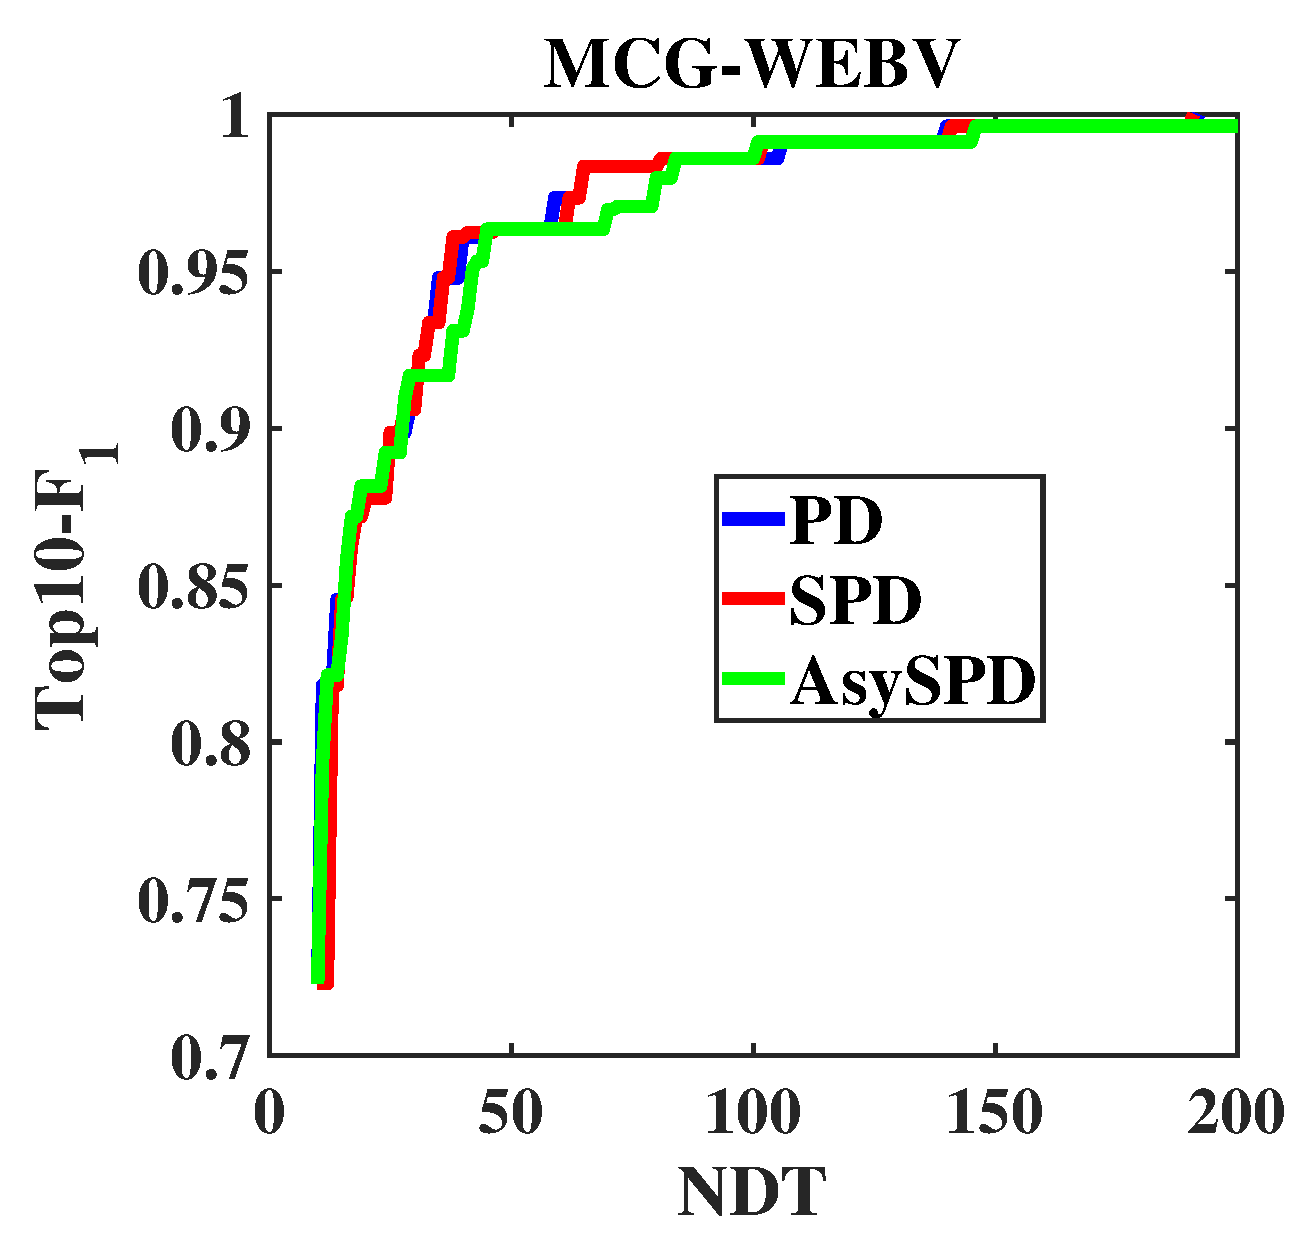
\includegraphics[width=\textwidth,height=0.95\textwidth]{MCG_Top10_Asy}
      \caption{}
      \label{fig:MCG_Top10_Asy}
    \end{subfigure}%
    % ~% add desired spacing
    \begin{subfigure}[b]{0.5\textwidth}
      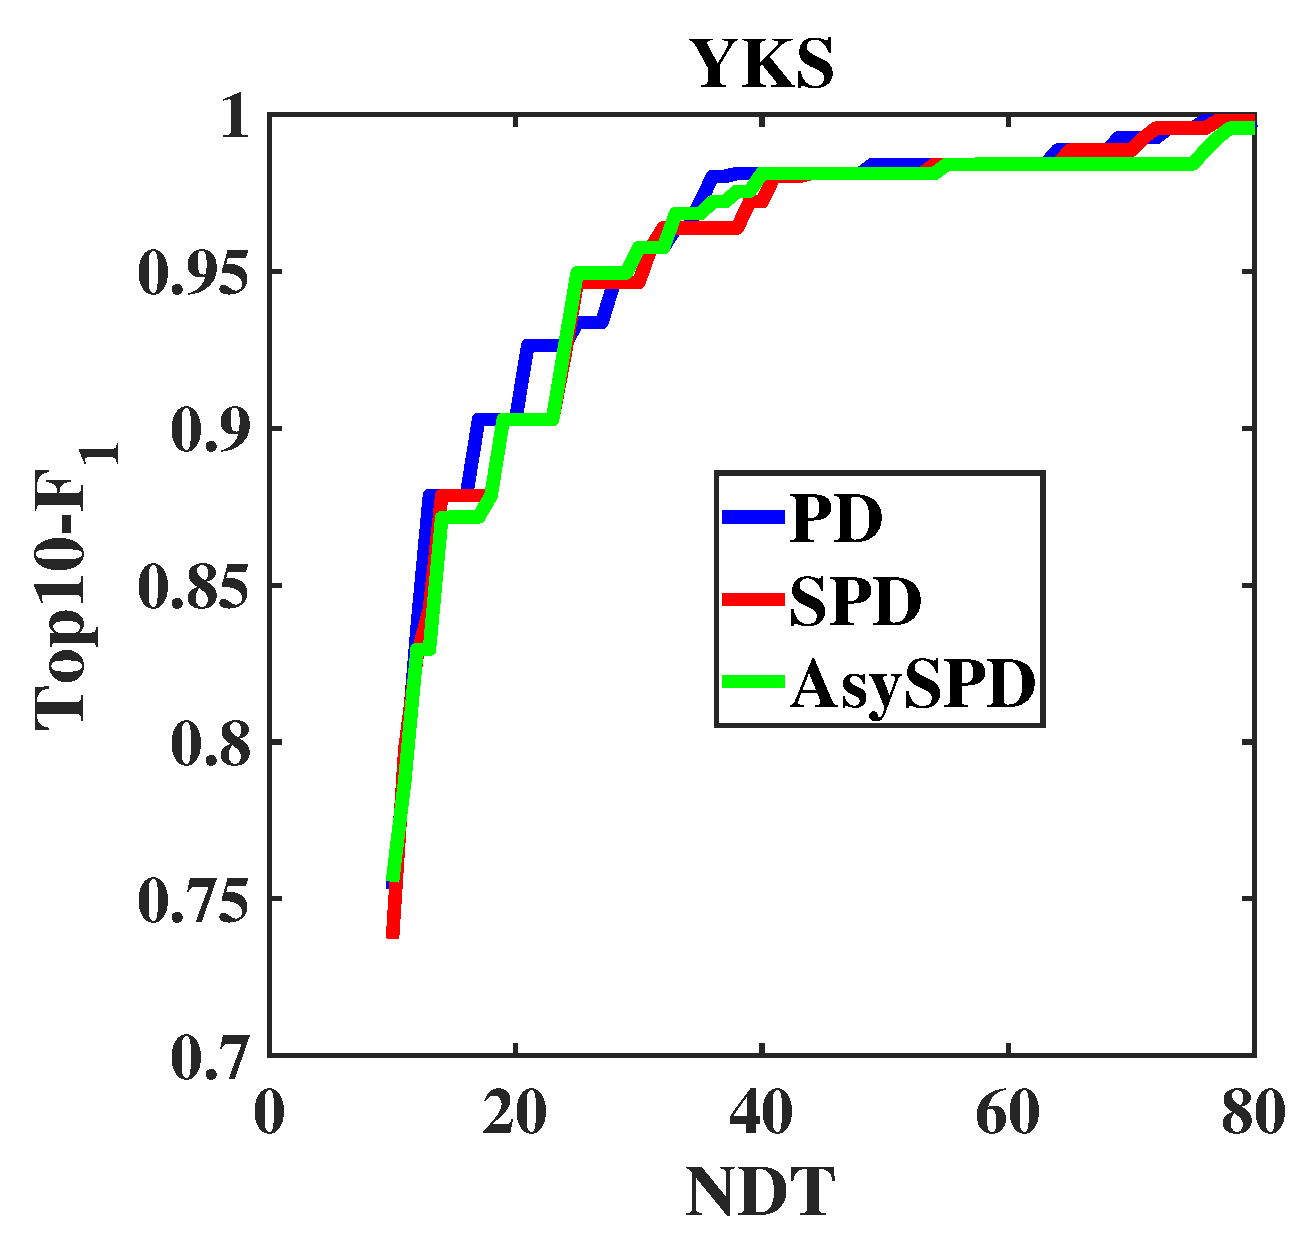
\includegraphics[width=\textwidth,height=0.95\textwidth]{YKS_Top10_Asy}
      \caption{}
      \label{fig:YKS_Top10_Asy}
    \end{subfigure}
    \caption{使用Top10-$F_1$ v.s. $NDT$对比SPD和AsySPD算法}
    \label{fig:MCG_YKS_Top10_AsySPD}
\end{figure}



\section{小结}

在本章中,我们提出了一种SPD算法,将随机优化最小化原则应用到PD算法中,从而能够优雅地处理大规模网络数据的话题检测问题。SPD算法迭代的利用小批量样本来更新目标函数的上界代理函数,同时最小化该代理函数,从而单调地驱使目标函数值下降。应用过程中注意到话题检测的特殊场景:一小批样本只能更新一部分话题的权重,而传统的随机梯度下降中的小批量样本能更新所有的权重。所以,在每次更新时,只更新那些被当前批样本影响到的话题。最终在话题检测效果方面,我们通过实验展示了我们的算法可以取得和当前最好的话题检测算法相似的性能。同时,我们构造了一个较大规模的人工数据集来验证我们算法高效的收敛速度。最后,我们提出AsySPD算法来实现SPD算法的异步并行更新。